\chapter{Fundamentos teóricos}

Este capítulo presenta los conceptos esenciales sobre la interpretabilidad en inteligencia artificial y su relevancia en aplicaciones críticas donde la transparencia es fundamental. Se describen los enfoques intrínsecos para mejorar la interpretabilidad, como los árboles de decisión (DT) y los Interpretable Decision Sets (IDS), junto con técnicas como la sparsidad, simulabilidad, modularidad y parsimonia. También se exploran métodos basados en reglas y se discuten los factores que influyen en la percepción de interpretabilidad y la confianza del usuario, proporcionando el marco teórico necesario para este TFM.

\section{Introducción a la Interpretabilidad}

La interpretabilidad en el campo de la inteligencia artificial (IA) se define como la capacidad de explicar o presentar los resultados de un sistema de aprendizaje automático de manera comprensible para los seres humanos. Es fundamental para garantizar que se cumplan criterios como la equidad, la privacidad, la fiabilidad, la robustez, la causalidad, la usabilidad y la confianza. De este modo, permite a los usuarios entender cómo funcionan los algoritmos y verificar si estos cumplen con los objetivos esperados \cite{doshi2017towards, gunning2019xai}.

A diferencia de la explicabilidad, que se enfoca en proporcionar explicaciones posteriores al desarrollo de los modelos (post-hoc), la interpretabilidad basada en modelos implica un diseño intencional desde la etapa de modelado para que sean comprensibles para los usuarios. Esto puede lograrse mediante la construcción de modelos intrínsecamente interpretables, como los árboles de decisión, que ofrecen claridad sobre las relaciones aprendidas a partir de los datos. Sin embargo, este enfoque presenta el reto de equilibrar la simplicidad del modelo con su precisión predictiva, además de lidiar con posibles sesgos en los datos o en los métodos explicativos utilizados \cite{murdoch2019interpretable, Kaur-2020}.

Existen dos enfoques principales para abordar la interpretabilidad:

\begin{itemize}
    \item \textit{Interpretabilidad local:} Se centra en explicar la predicción del modelo para una instancia específica. Responde preguntas como: "¿Por qué se tomó esta decisión para este dato?". Técnicas como LIME (Local Interpretable Model-agnostic Explanations) muestran qué características del dato son más relevantes para una predicción individual \cite{doshi2017towards, gilpin2018explaining}. Es útil en situaciones donde se necesita entender decisiones individuales, como en diagnósticos médicos o aprobaciones de crédito.

    \item \textit{Interpretabilidad global:} Busca comprender el comportamiento general del modelo en todo el conjunto de datos. Responde a preguntas como: "¿Cómo toma decisiones el modelo en general?" o "¿Qué patrones ha aprendido el modelo?". Métodos como los árboles de decisión y los modelos aditivos generalizados (GAMs) ofrecen una visión global, permitiendo observar cómo las predicciones varían según las características de los datos \cite{doshi2017towards, Kaur-2020}. Es crucial en aplicaciones que requieren entender las reglas generales del modelo, como en políticas públicas o investigaciones científicas.
\end{itemize}

Ambos enfoques son complementarios y se aplican en diferentes contextos. Mientras que la \textit{interpretabilidad local} facilita la comprensión de decisiones individuales, la \textit{interpretabilidad global} proporciona una visión más amplia del funcionamiento del modelo, lo cual es esencial para su validación y aceptación en aplicaciones críticas \cite{gilpin2018explaining, doshi2017towards, Kaur-2020}.

En este TFM, la interpretabilidad se analizará en el contexto de modelos de decisión interpretables, específicamente en los \textit{Interpretable Decision Sets} (IDS) y los árboles de decisión (DT). Se explorará cómo la estructura del modelo, la presentación de resultados y otros factores influyen en la percepción de interpretabilidad y en la capacidad de los usuarios para detectar errores.


\section{Criterios de interpretabilidad}

Esta sección se basa en los trabajos de Murdoch et al. (2019) \cite{murdoch2019interpretable} y Rudin (2019) \cite{Rudin-2019}, quienes destacan, desde diferentes perspectivas, la importancia de utilizar modelos de decisión que sean inherentemente interpretables en aplicaciones donde la transparencia es crucial, como la medicina, la justicia o la toma de decisiones críticas en entornos regulatorios. 

Los modelos de caja negra, utilizados en decisiones de alto riesgo, pueden tener consecuencias negativas significativas debido a la falta de transparencia y a la dificultad para interpretar sus resultados. Por ello, ambos autores recomiendan el uso de modelos interpretables que proporcionen explicaciones fieles y comprensibles, en lugar de depender de explicaciones post hoc.

Según estos estudios, es más efectivo diseñar modelos que sean interpretables desde el principio, ya que esto evita las complicaciones asociadas con la explicación de modelos complejos. Para alcanzar esta interpretabilidad, se pueden utilizar varios enfoques intrínsecos, tales como la sparsidad, la simulabilidad, y la modularidad. A continuación, se exploran estos tres enfoques y sus beneficios en el diseño de modelos interpretables.

\subsection{Sparsidad}

La sparsidad implica reducir el número de parámetros no nulos en un modelo, lo que facilita la comprensión del papel específico de cada variable en las predicciones. Este enfoque es particularmente útil en casos donde se sabe que la relación subyacente depende de un conjunto limitado de señales significativas. Por ejemplo, los modelos lineales, como la regresión LASSO (Least Absolute Shrinkage and Selection Operator), o métodos como el sparse coding, aplican técnicas de penalización para mantener la simplicidad del modelo sin comprometer significativamente la precisión predictiva \cite{kukreja2006least}. Esta reducción en complejidad no solo mejora la interpretabilidad, sino que también puede ayudar a evitar el sobreajuste al destacar características verdaderamente relevantes.

La regresión LASSO se define mediante la siguiente ecuación \cite{kukreja2006least}:

\begin{equation}
\min_{\theta} \left( \frac{1}{2} \|Z - \Phi \theta \|_2^2 + \lambda \|\theta\|_1 \right),
\end{equation}

donde \(Z\) es el vector de las salidas observadas, \(\Phi\) es la matriz de regresores (características), \(\theta\) es el vector de parámetros desconocidos del modelo, \(\| \cdot \|_2\) denota la norma \(L_2\), y \(\| \cdot \|_1\) denota la norma \(L_1\).

La sparsidad se promueve a través del término de penalización \(\lambda \|\theta\|_1\), que reduce algunos de los coeficientes \(\theta\) a cero. Este enfoque favorece modelos más simples y parsimoniosos, mejorando la interpretabilidad al centrarse únicamente en las características más relevantes.

\begin{figure}[H]
    \centering
    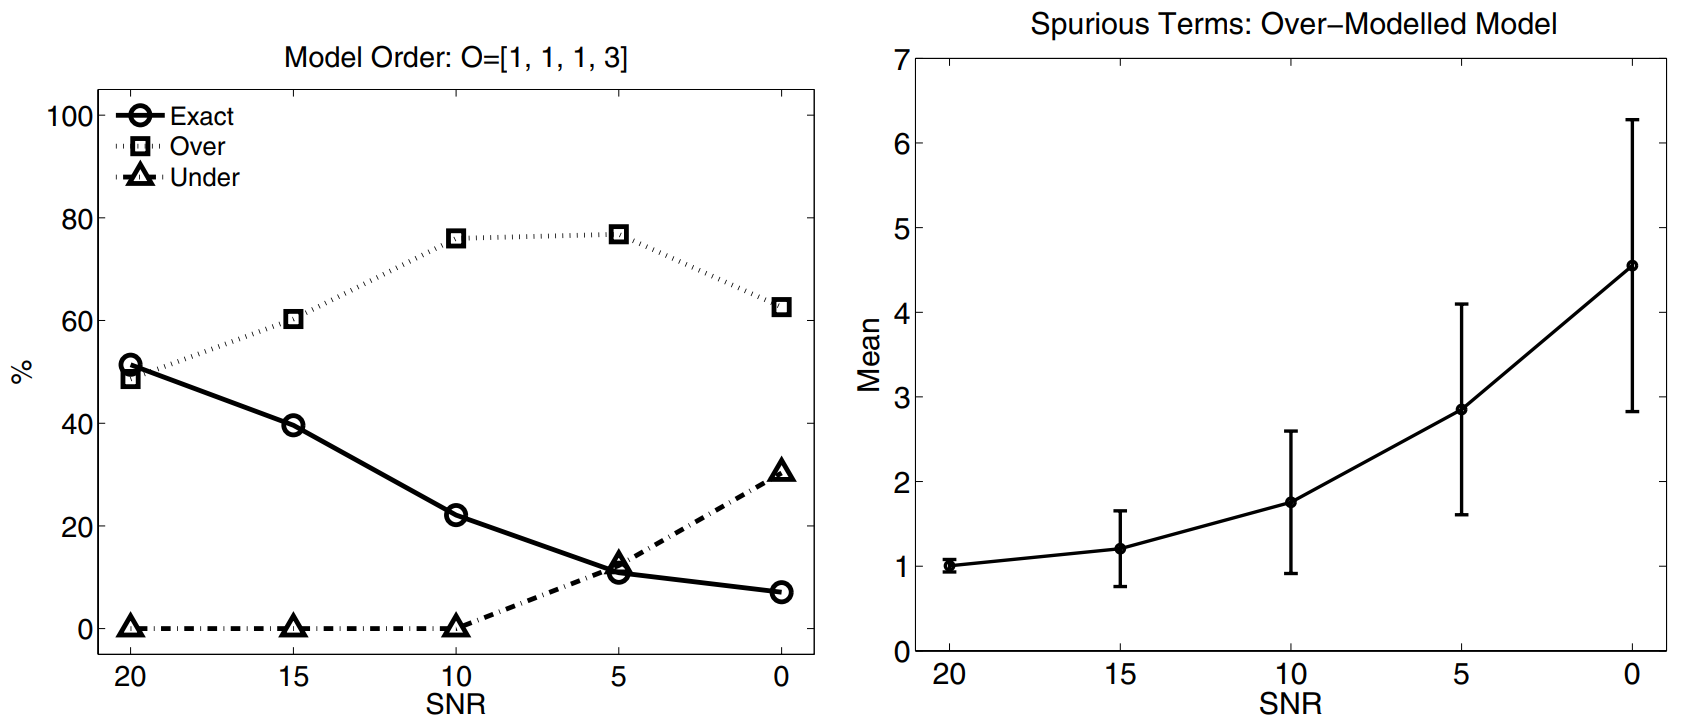
\includegraphics[width=0.7\textwidth]{include/lasso.png}
    \caption{Relación entre sparsidad y selección de modelos utilizando LASSO. El gráfico de la izquierda muestra la tasa de selección de modelos exactos (círculos), sobre-modelados (cuadrados) y sub-modelados (triángulos) en función del nivel de ruido en la señal (SNR). Un modelo exacto tiene solo las variables relevantes, mientras que un sobre-modelado incluye variables adicionales innecesarias (términos espurios) y un sub-modelado omite variables relevantes. El gráfico de la derecha muestra la media y desviación estándar del número de términos espurios seleccionados en modelos sobre-modelados, destacando cómo LASSO minimiza la inclusión de estas variables irrelevantes, promoviendo así la sparsidad y la interpretabilidad del modelo. Adaptado de \cite{kukreja2006least}.}
    \label{fig:lasso}
\end{figure}


\subsection{Simulabilidad}

Por otro lado, la simulabilidad se refiere a la capacidad de un modelo para ser reproducido y comprendido fácilmente por un ser humano. Modelos como los árboles de decisión y las listas de reglas ``si-entonces'' ejemplifican esta característica, ya que permiten seguir paso a paso el proceso de toma de decisiones del modelo. Este enfoque es especialmente valioso en contextos donde las decisiones deben ser comprensibles para personas no expertas, como en aplicaciones médicas, donde tanto los pacientes como los profesionales de la salud necesitan entender las recomendaciones del modelo.

\begin{figure}[h!]
\centering
\begin{tikzpicture}
    \Tree [.{¿X1 > 5?}
        [.{Sí} [.{Y = Clase A} ] ]
        [.{No} 
            [.{¿X2 < 3?}
                [.{Sí} [.{Y = Clase B} ] ]
                [.{No} [.{Y = Clase C} ] ]
            ]
        ]
    ]
\end{tikzpicture}
\caption{Árbol de decisión basado en \cite{murdoch2019interpretable} que ejemplifica la simulabilidad al dividir el espacio de características en regiones de decisión claras mediante reglas "si-entonces". Cada nodo representa una pregunta sobre las características (\(X_1\) y \(X_2\)), y las ramas llevan a decisiones simples ("Sí" o "No"), facilitando que cualquier usuario pueda seguir y reproducir el proceso de toma de decisiones del modelo.}
\label{fig:decision_tree}
\end{figure}

\subsection{Modularidad}

La modularidad es un enfoque clave en modelos interpretables, ya que permite descomponer el modelo en partes significativas que se pueden interpretar de forma independiente. Este enfoque es particularmente útil en modelos complejos, donde los subcomponentes o módulos tienen un significado interpretativo claro. 

Por ejemplo, los Modelos Aditivos Generalizados (GAMs)\cite{hastie2017generalized}, como el Explainable Boosting Machine (EBM) \cite{murdoch2019interpretable}, restringen las relaciones entre las variables a una forma aditiva, lo que facilita la interpretación de cada término individual. Esto significa que cada función en el modelo representa el efecto de un predictor específico en la predicción final, y estos efectos se pueden analizar de manera aislada para comprender su contribución individual.

La ecuación de un GAM se puede expresar como:

\begin{equation}
g(\mu) = \beta + f_1(x_1) + \cdots + f_m(x_m)
\end{equation}

donde \(g(\mu)\) es la función de enlace, \(\beta\) es el término independiente, y \(f_i(x_i)\) son funciones suaves que representan el efecto de cada predictor \(x_i\).

\begin{figure}[H]
    \centering
    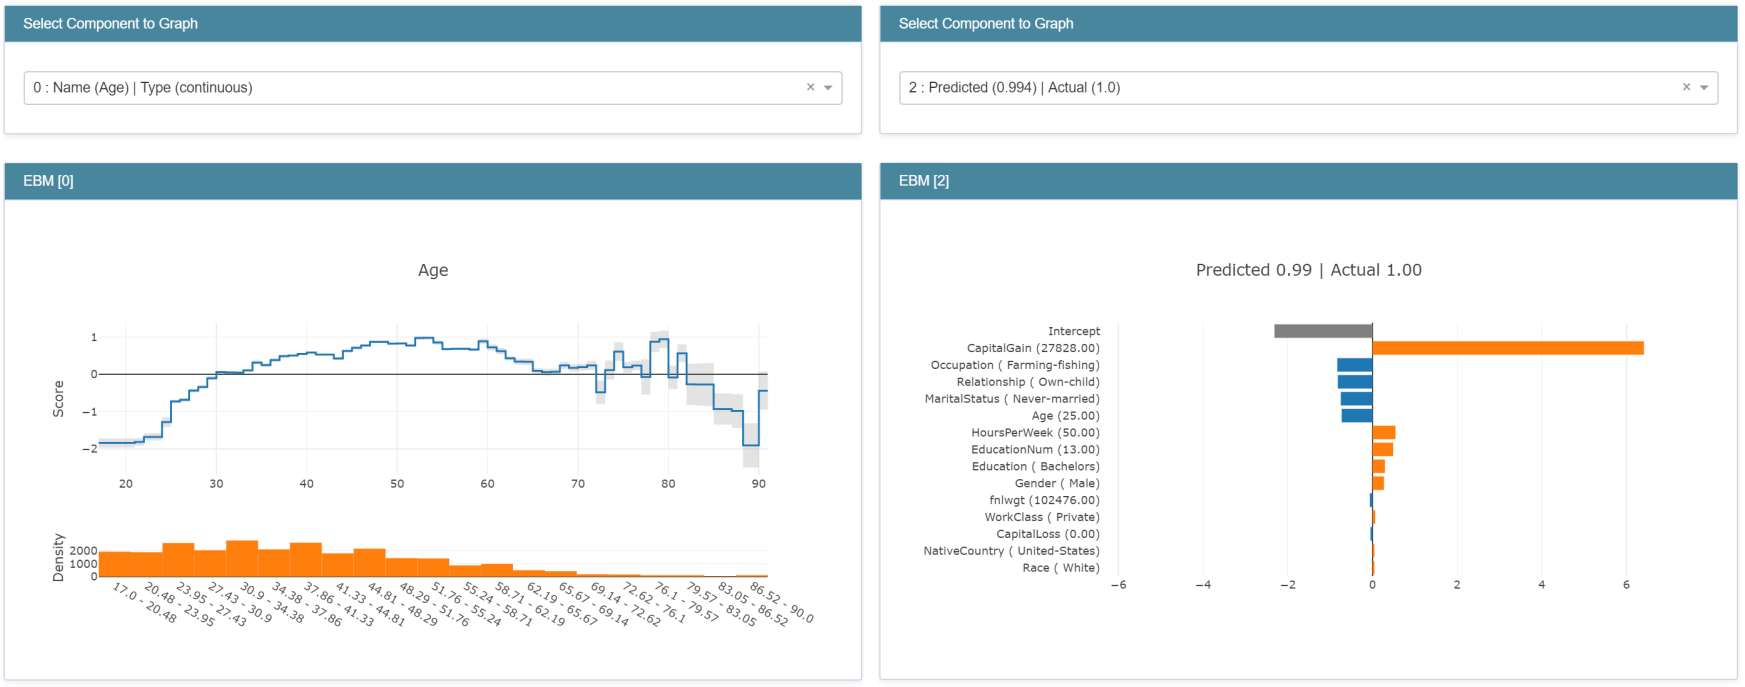
\includegraphics[width=1\textwidth]{include/modularity.png}
    \caption{Ejemplo de modularidad en un modelo aditivo como el EBM. Izquierda: La función \( f_{\text{Age}} \) muestra cómo la característica 'Edad' afecta la predicción final. Derecha: Descomposición de una predicción individual, donde se destaca cómo cada característica contribuye de manera independiente, con 'CapitalGain' dominando la predicción. Adaptado de \cite{murdoch2019interpretable}.}
    \label{fig:modularidad_ebm}
\end{figure}

\subsection{Parsimonía}

La parsimonia se refiere a la simplicidad de un modelo al utilizar el mínimo número de parámetros o términos necesarios para capturar la dinámica de un sistema. Esto facilita la interpretabilidad y la generalización del modelo, ya que reduce la complejidad y ayuda a evitar sobreajustes. Según Kutz y Brunton (2022), promover la parsimonia en el aprendizaje automático, especialmente en modelos informados por la física, resulta en modelos más interpretables y físicamente coherentes, permitiendo una mejor generalización a nuevos escenarios.

\begin{figure}[H]
    \centering
    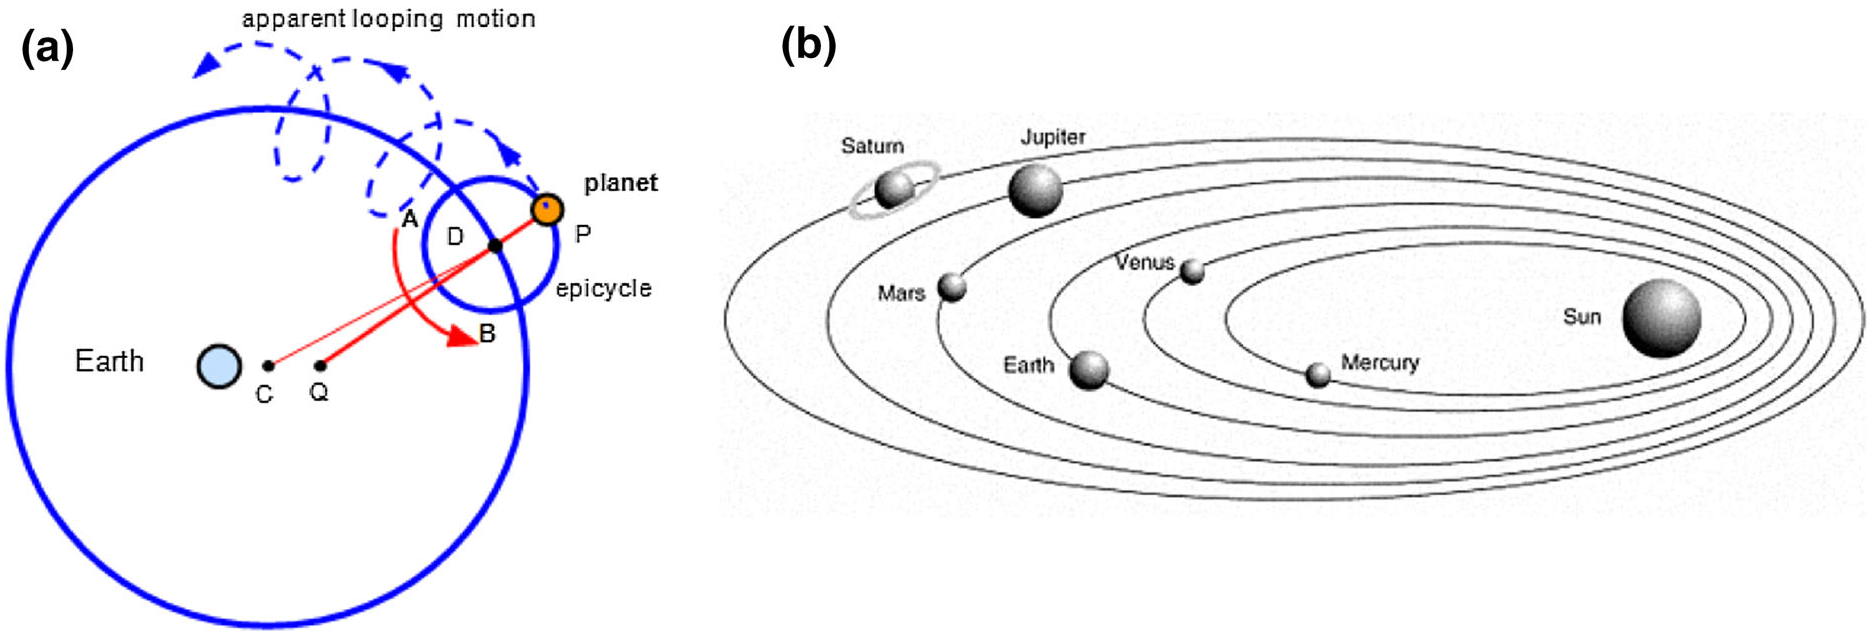
\includegraphics[width=1\textwidth]{include/solar.PNG}
    \caption{Comparación entre dos modelos astronómicos que ilustran el principio de parsimonía: (a) El modelo ptolemaico describe el movimiento planetario con epiciclos y deferentes, donde el ángulo azimutal del planeta se calcula mediante \(\alpha(t) = \Omega t - \sin^{-1} \left( \frac{CE}{R} \sin(\Omega t) \right)\) \cite{rushkin2015optimizing}, lo que implica una mayor complejidad debido a la necesidad de múltiples parámetros; (b) El modelo heliocéntrico de Copérnico, refinado por Newton, utiliza una ley de gravitación universal más simple, \( F = G \frac{m_1 m_2}{r^2} \), que requiere menos supuestos y es más parsimonioso. Imagen adaptada de \cite{kutz2022parsimony}.}
    \label{fig:parsimonia}
\end{figure}

\subsection{Subgrupos: Métodos Contrastivos y Emergentes}

Además de los enfoques intrínsecos como la sparsidad, la simulabilidad, la modularidad y la parsimonia, los métodos basados en reglas también emplean técnicas específicas para mejorar la interpretabilidad mediante la identificación de patrones diferenciados en los datos. Un enfoque destacado es el \textit{descubrimiento de subgrupos}, que busca encontrar segmentos de datos que sean relevantes o interesantes con respecto a una variable de interés.

A diferencia de métodos como las Máquinas de Soporte Vectorial o Redes Neuronales, que se enfocan en maximizar la precisión de la clasificación de ejemplos individuales, los métodos basados en reglas, como el descubrimiento de subgrupos, se centran en caracterizar las clases a través de sus relaciones con otras entidades presentes en los datos \cite{duda-2000}. Estos métodos no solo se preocupan por la precisión de la predicción, sino también por la claridad y comprensibilidad de las relaciones aprendidas, lo cual es esencial para la interpretabilidad \cite{Herrera-2010}.

El \textit{descubrimiento de subgrupos}, un concepto ampliamente utilizado en minería de datos, consiste en identificar segmentos de la población que sean estadísticamente relevantes según ciertos criterios. Estos segmentos se definen mediante reglas del tipo “si-condición(es)-entonces-clase”, que permiten describir de forma comprensible cómo se agrupan los datos respecto a una propiedad específica \cite{Wrobel-2001, Herrera-2010}. Este paradigma incluye tres enfoques principales:

\begin{enumerate}
    \item \textit{Descubrimiento de subgrupos}: Este método busca identificar subgrupos dentro del conjunto de datos que tengan una alta probabilidad de cumplir con una determinada característica o condición de interés. Por ejemplo, en un estudio médico, puede identificar pacientes con síntomas similares que tienen una alta probabilidad de padecer una enfermedad específica.

    \item \textit{Conjunto de contraste}: Este enfoque se centra en encontrar pares de atributos y valores que sean únicos para cada grupo o clase. Su objetivo es maximizar la diferenciación entre clases, destacando atributos específicos que caracterizan exclusivamente a cada clase. Por ejemplo, en los árboles de decisión, se busca que cada nodo defina claramente las fronteras entre las diferentes clases (ver Figura \ref{fig:decision_tree}).

    \item \textit{Patrón emergente}: Se enfoca en extraer subgrupos en los que las frecuencias relativas de la variable objetivo varían de manera significativa entre los distintos grupos. Utiliza listas de decisión y métodos centrados en la "cobertura" de reglas para identificar los atributos que son más representativos o influyentes para una clase específica. Este enfoque es útil para descubrir reglas o patrones que puedan ser menos evidentes pero importantes para la comprensión del modelo (ver Figura \ref{fig:modularidad_ebm}).
\end{enumerate}

En general, estos algoritmos utilizan heurísticas para aproximar un conjunto óptimo de reglas, lo que significa que introducen ciertos supuestos sobre la estructura de los datos para hacer el problema manejable en tiempo polinomial. Estas técnicas ayudan a construir modelos que no solo sean precisos, sino también comprensibles para los usuarios finales, permitiendo una mejor toma de decisiones basada en las interpretaciones claras proporcionadas por las reglas generadas.

\subsection{Contexto y Audiencia}

Finalmente, la elección del enfoque interpretativo depende en gran medida del contexto del problema y de la audiencia objetivo. En aplicaciones donde la precisión predictiva es menos crítica que la interpretabilidad, como en auditorías de modelos para asegurar la equidad, se prefieren modelos más simples y transparentes. En cambio, en situaciones que exigen alta precisión, se pueden considerar métodos post hoc para interpretar modelos más complejos, asegurando así un equilibrio adecuado entre interpretabilidad y precisión.

\begin{figure}[H]
    \centering
    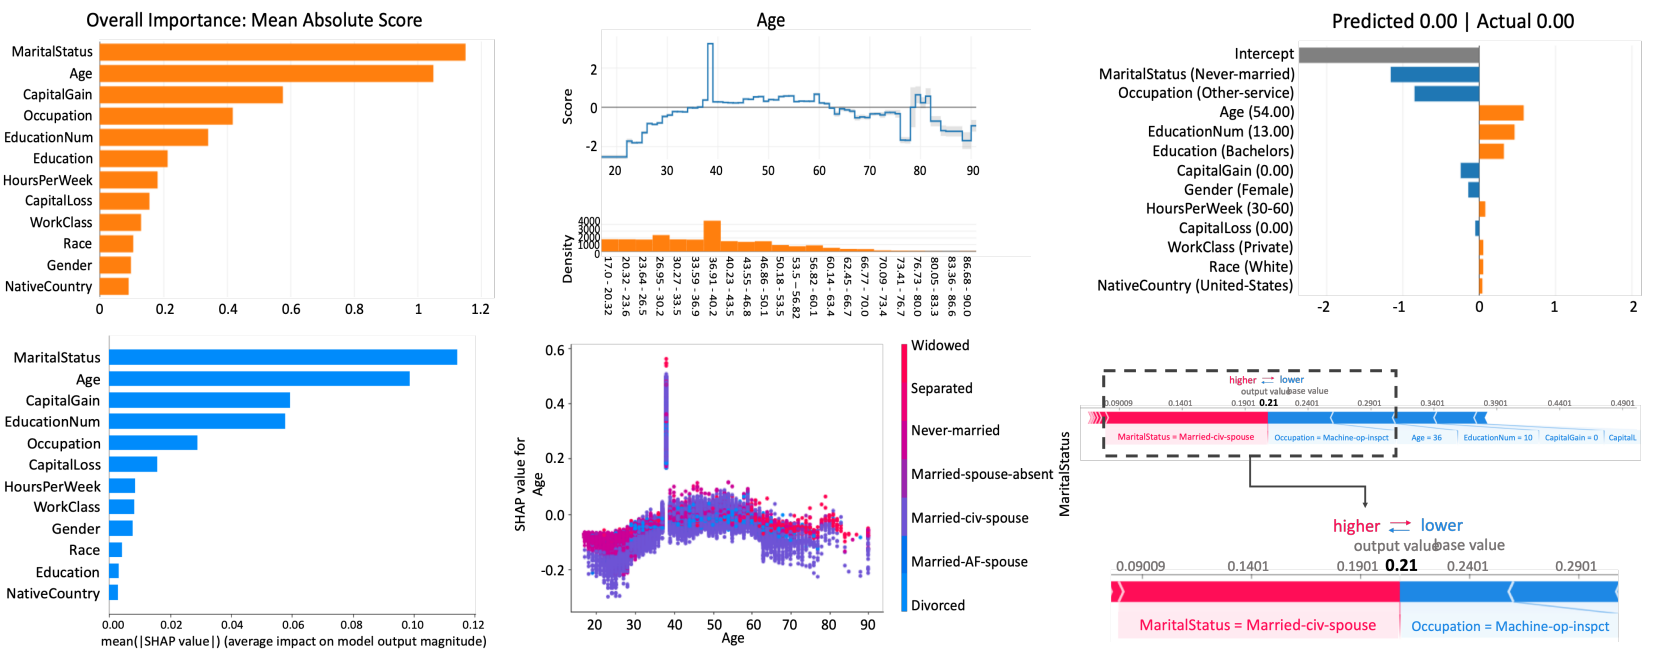
\includegraphics[width=1\textwidth]{include/contexto.PNG}
    \caption{Las visualizaciones de GAM (arriba) y SHAP (abajo), adaptadas de \cite{Kaur-2020} y generadas por InterpretML \cite{nori2019interpretml}, muestran cómo diferentes enfoques interpretativos se ajustan a diversas audiencias y contextos. Las explicaciones globales (columna izquierda) ayudan a científicos de datos a identificar las variables más influyentes en el modelo; los gráficos de componentes o de dependencia (columna central) son útiles para que analistas de negocio interpreten el impacto de factores específicos, como edad o ingreso, en la puntuación crediticia; y las explicaciones locales (columna derecha) son cruciales en medicina personalizada para justificar decisiones como la recomendación de un tratamiento específico.}
    \label{fig:contexto_audiencia}
\end{figure}

\section{Modelos de Decisión Interpretables}

A continuación, se presentan los tres modelos interpretables con los que evaluaremos la interpretabilidad en este TFM.

\subsection{Árboles de Decisión (DT)}

Esta sección se basa en los trabajos de Mienye et al. (2024) \cite{mienye2024survey} y Duda et al. (2000) \cite{duda-2000}, quienes proporcionan un análisis exhaustivo de los conceptos, algoritmos y aplicaciones de los Árboles de Decisión (DT). Los DT son modelos de aprendizaje supervisado utilizados tanto para tareas de clasificación como de regresión. Un árbol de decisión se construye dividiendo iterativamente un conjunto de datos en subconjuntos más pequeños basados en reglas de decisión derivadas de las características de los datos. Cada nodo interno del árbol representa una característica o atributo, mientras que cada rama representa una regla de decisión y cada hoja final una decisión o resultado.

\begin{figure}[H]
    \centering
    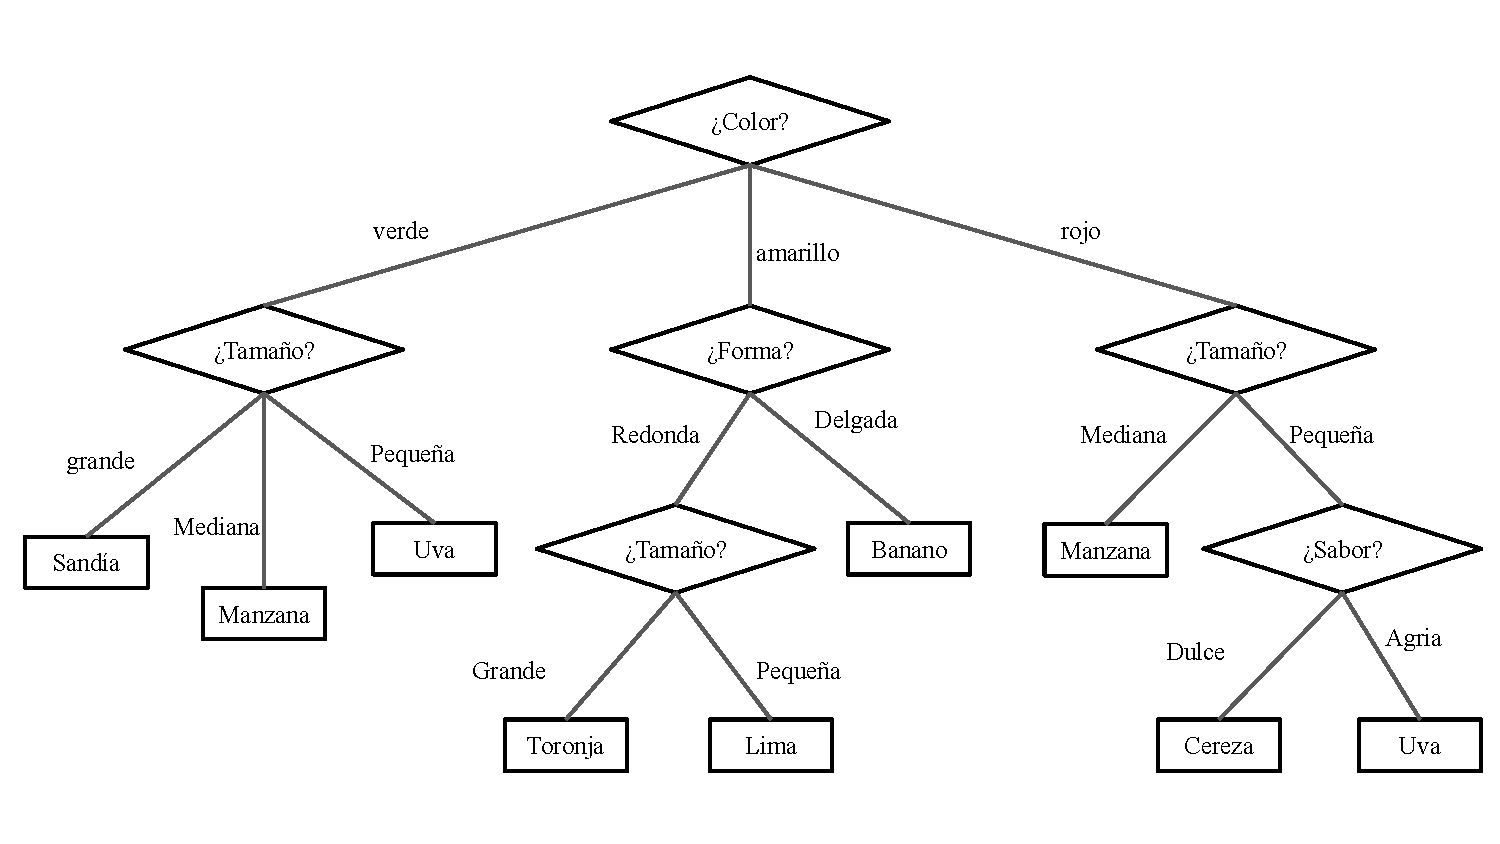
\includegraphics[width=\textwidth]{include/arbol decision.pdf}
    \caption{Ilustración de un árbol de decisión basada en técnicas de clasificación no paramétricas. Adaptada de \cite{duda-2000}, Capítulo 4. Los árboles de decisión son fáciles de interpretar cuando son pequeños, pero pueden volverse complejos y difíciles de validar a medida que crecen \cite{Liu-2015}. }
    \label{fig:decision-tree}
\end{figure}

\begin{figure}[H]
\centering
\fbox{
\begin{minipage}{0.9\linewidth}
\scriptsize
\textbf{si} \textcolor{blue}{color} = \textcolor{blue}{verde} \textbf{y} \textcolor{blue}{tamaño} = \textcolor{blue}{grande} \textbf{entonces} \textcolor{red}{Sandía} \\[0.3em]
\textbf{si} \textcolor{blue}{color} = \textcolor{blue}{verde} \textbf{y} \textcolor{blue}{tamaño} = \textcolor{blue}{mediana} \textbf{entonces} \textcolor{red}{Manzana} \\[0.3em]
\textbf{si} \textcolor{blue}{color} = \textcolor{blue}{verde} \textbf{y} \textcolor{blue}{tamaño} = \textcolor{blue}{pequeña} \textbf{entonces} \textcolor{red}{Uva} \\[0.3em]
\textbf{si} \textcolor{blue}{color} = \textcolor{blue}{amarillo} \textbf{y} \textcolor{blue}{forma} = \textcolor{blue}{redonda} \textbf{y} \textcolor{blue}{tamaño} = \textcolor{blue}{grande} \textbf{entonces} \textcolor{red}{Toronja} \\[0.3em]
\textbf{si} \textcolor{blue}{color} = \textcolor{blue}{amarillo} \textbf{y} \textcolor{blue}{forma} = \textcolor{blue}{redonda} \textbf{y} \textcolor{blue}{tamaño} = \textcolor{blue}{pequeña} \textbf{entonces} \textcolor{red}{Lima} \\[0.3em]
\textbf{si} \textcolor{blue}{color} = \textcolor{blue}{amarillo} \textbf{y} \textcolor{blue}{forma} = \textcolor{blue}{delgada} \textbf{entonces} \textcolor{red}{Banano} \\[0.3em]
\textbf{si} \textcolor{blue}{color} = \textcolor{blue}{rojo} \textbf{y} \textcolor{blue}{tamaño} = \textcolor{blue}{mediana} \textbf{entonces} \textcolor{red}{Manzana} \\[0.3em]
\textbf{si} \textcolor{blue}{color} = \textcolor{blue}{rojo} \textbf{y} \textcolor{blue}{tamaño} = \textcolor{blue}{pequeña} \textbf{y} \textcolor{blue}{sabor} = \textcolor{blue}{dulce} \textbf{entonces} \textcolor{red}{Cereza} \\[0.3em]
\textbf{si} \textcolor{blue}{color} = \textcolor{blue}{rojo} \textbf{y} \textcolor{blue}{tamaño} = \textcolor{blue}{pequeña} \textbf{y} \textcolor{blue}{sabor} = \textcolor{blue}{agrio} \textbf{entonces} \textcolor{red}{Uva}
\end{minipage}
}
\caption{Reglas de decisión basadas en el árbol de decisión de la Figura \ref{fig:decision-tree}.}
\label{fig:decision-rules}
\end{figure}

El entrenamiento de un árbol es un proceso recursivo que comienza con todos los datos en la raíz y divide sucesivamente los nodos según la mejor característica, repitiendo el proceso en cada nodo hijo \cite{duda-2000}. Uno de los algoritmos más utilizados para construir árboles de decisión es el ID3, que selecciona la característica que proporciona la mayor ganancia de información. A continuación se presenta el algoritmo:

\begin{algorithm}[H]
\caption{Algoritmo ID3 para Árbol de Decisión}
\KwIn{Conjunto de datos de entrenamiento $D = \{(x_1, y_1), (x_2, y_2), \ldots, (x_m, y_m)\}$}
\KwOut{Árbol de decisión $T$}

\SetKwFunction{FMain}{ID3}
\SetKwProg{Fn}{Función}{:}{}
\Fn{\FMain{$D$}}{
    \If{$D$ está vacío}{
        \Return{un nodo terminal con clase por defecto $c_{default}$}
    }
    \If{todas las instancias en $D$ tienen la misma etiqueta de clase $y$}{
        \Return{un nodo terminal con clase $y$}
    }
    \If{el conjunto de atributos $J$ está vacío}{
        \Return{un nodo terminal con la clase más frecuente en $D$}
    }
    Seleccionar el atributo $f$ que mejor divide los datos usando ganancia de información\;
    Crear un nodo de decisión para $f$\;
    \For{cada valor posible $b_i$ de $f$}{
        Crear una rama para $b_i$\;
        Sea $D_i$ el subconjunto de $D$ donde $x_i = b_i$\;
        Recursivamente construir el subárbol para $D_i$\;
        Adjuntar el subárbol a la rama para $b_i$\;
    }
    \Return{el nodo de decisión}
}
\end{algorithm}

Uno de los criterios más comunes para dividir los nodos es la ganancia de información, definida como:

\begin{equation}
\text{Ganancia de Información} = I(p) - \sum_{i} \frac{|p_i|}{|p|} I(p_i),
\end{equation}

donde \( I(p) \) es la entropía del conjunto de datos original, y \( I(p_i) \) es la entropía del subconjunto resultante después de la división.

Otro criterio utilizado es el índice de Gini:

\begin{equation}
\text{Índice de Gini} = 1 - \sum_{i} p_i^2,
\end{equation}

donde \( p_i \) representa la proporción de observaciones de la clase \( i \) en el nodo.

\subsection{Listas de decisión}

Las listas de decisión son una representación para funciones Booleanas construidas como secuencias ordenadas de predicados lógicos del tipo “si [condición(es)] entonces [clase]” seguida de otras condiciones adicionales (e.g., “más si [condición(es)] entonces [clase]”). Las condiciones corresponden a predicados sobre las características del problema de clasificación (los \emph{features}) \cite{Liu-2015, Letham-2015, Rivest-1987}.

\begin{figure}[H]
\centering
\begin{tikzpicture}[node distance=2.5cm, auto]
    % Nodos del diagrama
    \node (decision1) [decision, align=center] {Género = ¿Hombre?\\Edad = ¿Adulto?};
    \node (decision2a) [decision, below left of=decision1, node distance=4cm, align=center] {Clase = ¿3ra?};
    \node (decision2b) [decision, below right of=decision1, node distance=4cm, align=center] {Clase = ¿1ra?};
    \node (victim) [process, below left of=decision2a, yshift=-0.4cm] {Víctima};
    \node (survivor) [process, below of=decision1, yshift=-2.5cm] {Sobreviviente};
    \node (survivor2) [process, below right of=decision2b, yshift=-0.4cm] {Sobreviviente};

    % Conectar los nodos con flechas
    \draw [arrow] (decision1) -- node[anchor=east, pos=0.2] {Sí} (decision2a);
    \draw [arrow] (decision1) -- node[anchor=west, pos=0.2] {No} (decision2b);
    \draw [arrow] (decision2a) -- node[anchor=east, pos=0.5] {Sí} (victim);
    \draw [arrow] (decision2a) -- node[anchor=west, pos=0.5] {No} (survivor);
    \draw [arrow] (decision2b) -- node[anchor=west, pos=0.2] {Sí} (survivor2);
    \draw [arrow] (decision2b) -- node[anchor=west, pos=0.5] {No} (survivor);
\end{tikzpicture}
\caption{Ejemplo de lista de decisión. Adaptado de \cite{Letham-2015}. Se muestra entrenado con el conjunto de datos del Titanic}
\label{fig:decision-list-diagram}
\end{figure}

\begin{figure}[H]
\centering
\fbox{
\begin{minipage}{0.9\linewidth}
\scriptsize
\textbf{si} \textcolor{blue}{género} = \textcolor{blue}{hombre} \textbf{y} \textcolor{blue}{edad} = \textcolor{blue}{adulto} \textbf{entonces} \textcolor{red}{víctima} \\[0.3em]
\textbf{si no, si} \textcolor{blue}{clase} = \textcolor{blue}{3ra} \textbf{entonces} \textcolor{red}{víctima} \\[0.3em]
\textbf{si no, si} \textcolor{blue}{clase} = \textcolor{blue}{1ra} \textbf{entonces} \textcolor{red}{sobreviviente} \\[0.3em]
\textbf{si no,} \textcolor{red}{sobreviviente}
\end{minipage}
}
\caption{Reglas de decisión basadas en el árbol de decisión de la Figura \ref{fig:decision-tree}.}
\end{figure}

A diferencia de otros métodos de aprendizaje automático como Máquinas de Soporte Vectorial, Bosques Aleatorios o Redes Neuronales, las listas de decisión ofrecen una explicación natural y sencilla para cada predicción, permitiendo que un experto entienda el mecanismo de decisión y razone sobre el resultado. Esto se considera una ventaja significativa de las listas de decisión \cite{Letham-2015}.

Además, las listas de decisión también ofrecen ventajas durante el proceso de entrenamiento cuando se comparan con otros métodos interpretables, como los árboles de decisión. Mientras que estos métodos utilizan algoritmos avaros, lo cual permite tiempos de entrenamiento cortos pero a costa de una reducción en el desempeño, las listas de decisión construyen modelos secuenciales más robustos, manteniendo una mayor capacidad explicativa \cite{Liu-2015}.

Gracias a su naturaleza “emergente,” las listas de decisión se construyen mediante reglas que particionan el espacio de características de manera más significativa. Por ejemplo, una lista de decisión de tamaño \(k\) (k-DL) utiliza reglas en forma de cláusulas conjuntas, donde cada regla \(r_i\) puede representarse matemáticamente como:

\[
r_i : \bigwedge_{j=1}^{m_i} (x_j = a_{ij}) \rightarrow y = c_i,
\]

donde \(x_j\) son los atributos, \(a_{ij}\) son los valores específicos de dichos atributos, y \(c_i\) es la clase asignada. Este enfoque garantiza la tratabilidad computacional del problema, explorando un mayor número de combinaciones posibles sin comprometer la eficiencia \cite{Letham-2015}.

En particular, basándonos en el trabajo de Rivest (1987), las listas de decisión son polinómicamente aprendibles. Esto significa que pueden ser aprendidas de manera eficiente usando algoritmos de aprendizaje, como se define en el marco teórico de Valiant (1984). Rivest demuestra que las listas de decisión de tamaño \(k\) (k-DL) pueden ser identificadas en tiempo polinómico mediante un algoritmo codicioso que selecciona en cada paso la regla que maximiza la ganancia de información:

\[
\Delta I = I(S) - I(S|A),
\]

donde \(I(S)\) es la entropía del conjunto de datos \(S\) y \(I(S|A)\) es la entropía después de dividir \(S\) usando el atributo \(A\) que mejor explica los datos restantes \cite{Rivest-1987}.

El algoritmo encuentra iterativamente reglas que cubren el mayor número de ejemplos de una misma clase, organizándolas en una lista secuencial. Cada regla se aplica en orden hasta que todos los ejemplos han sido clasificados.


\begin{algorithm}[H]
\caption{Algoritmo para Listas de Decisión}
\KwIn{Conjunto de datos de entrenamiento $D = \{(x_1, y_1), (x_2, y_2), \ldots, (x_m, y_m)\}$}
\KwOut{Lista de decisión $L$}

\SetKwFunction{FMain}{DecisionList}
\SetKwProg{Fn}{Función}{:}{}
\Fn{\FMain{$D$}}{
    $L \gets \emptyset$\;
    \While{$D$ no está vacío}{
        Encontrar la regla $r = (c, v)$ que cubra más ejemplos en $D$\;
        $L \gets L \cup \{r\}$\;
        Eliminar de $D$ los ejemplos cubiertos por $r$\;
    }
    \Return{L}
}
\end{algorithm}

\subsection{Conjuntos Interpretables de Decisión (IDS)}

Esta sección se basa en el trabajo de Lakkaraju et al. (2016) \cite{lakkaraju-2016}, quienes proponen un marco para construir modelos predictivos que son altamente precisos y al mismo tiempo altamente interpretables. Un conjunto de decisión es un conjunto de predicados lógicos asociados a una etiqueta de clase. Las variables de los predicados corresponden a los atributos del problema de clasificación (los \emph{features}). El predicado sigue la forma “si [condición(es)] entonces [clase]”. Cada predicado está compuesto por ítems (predicados más pequeños) unidos por conjunción. Se dice que el conjunto asigna una clase a un ejemplo si el predicado es verdadero. En caso de empates (varios predicados son verdaderos, pero asignan una clase diferente), se utiliza alguna regla de desempate, generalmente \emph{ad-hoc} para cada aplicación, como dar prioridad a la regla más específica o a la primera regla que se cumpla. La figura \ref{fig:ids-example} muestra un ejemplo de un conjunto de decisión, adaptado de este trabajo. 









\begin{figure}[H]
\centering
\begin{minipage}{0.4\textwidth}  % Define el ancho de la tabla
    % Leyenda con contorno
    \begin{tabular}{|l|}
    \hline
    \textbf{Definiciones} \\
    \hline
    1: Enfermedad Respiratoria = Sí \\
    2: Fumador = Sí \\
    3: Edad >= 50 \\
    4: Riesgo Cáncer de Pulmón = Sí \\
    5: Presión Sanguínea >= 0.3 \\
    6: Riesgo Depresión = Sí \\
    7: Depresiones Previas = Sí \\
    8: IMC >= 0.3 \\
    9: Seguro Médico = No \\
    10: Presión Sanguínea >= 0.3 \\
    11: Fumador = Sí \\
    12: IMC >= 0.2 \\
    13: Edad >= 60 \\
    14: Riesgo Diabetes = Sí \\
    15: IMC >= 0.4 \\
    16: Propensión a Infección >= 0.2 \\
    17: Visitas al Médico >= 0.4 \\
    18: Obesidad Infantil = Sí \\
    A: Cáncer de Pulmón \\
    B: Depresión \\
    C: Diabetes \\
    \hline
    \end{tabular}
\end{minipage}%
\hfill  % Espacio flexible entre la tabla y el diagrama
\begin{minipage}{0.55\textwidth}  % Define el ancho del diagrama
    \begin{tikzpicture}[node distance=1.5cm, auto]
        % Nodos comunes
        \node (cond1) [condition] {1};  % enfermedad respiratoria = sí
        \node (cond2) [condition, right of=cond1] {2};  % fumador = sí
        \node (cond3) [condition, right of=cond2] {3};  % edad >= 50

        \node (cond4) [condition, below of=cond1, node distance=1.5cm] {4};  % riesgo cáncer de pulmón = sí
        \node (cond5) [condition, right of=cond4] {5};  % presión sanguínea >= 0.3

        \node (cond6) [condition, below of=cond4, node distance=1.5cm] {6};  % riesgo depresión = sí
        \node (cond7) [condition, right of=cond6] {7};  % depresiones previas = sí

        \node (cond8) [condition, below of=cond6, node distance=1.5cm] {8};  % IMC >= 0.3
        \node (cond9) [condition, right of=cond8] {9};  % seguro médico = no
        \node (cond10) [condition, right of=cond9] {10};  % presión sanguínea >= 0.3

        \node (cond11) [condition, below of=cond8, node distance=1.5cm] {11};  % fumador = sí
        \node (cond12) [condition, right of=cond11] {12};  % IMC >= 0.2
        \node (cond13) [condition, right of=cond12] {13};  % edad >= 60

        \node (cond14) [condition, below of=cond11, node distance=1.5cm] {14};  % riesgo diabetes = sí
        \node (cond15) [condition, right of=cond14] {15};  % IMC >= 0.4
        \node (cond16) [condition, right of=cond15] {16};  % propensión a infección >= 0.2

        \node (cond17) [condition, below of=cond14, node distance=1.5cm] {17};  % visitas al médico >= 0.4
        \node (cond18) [condition, right of=cond17] {18};  % obesidad infantil = sí

        % Nodos de clases compartidos
        \node (classA) [class, right of=cond3, node distance=3cm] {A};  % cáncer de pulmón
        \node (classB) [class, right of=cond10, node distance=3cm] {B};  % depresión
        \node (classC) [class, right of=cond16, node distance=3cm] {C};  % diabetes

        % Conexiones
        \draw[arrow] (cond1) -- (cond2);
        \draw[arrow] (cond2) -- (cond3);
        \draw[arrow] (cond3) -- (classA);

        \draw[arrow] (cond4) -- (cond5);
        \draw[arrow] (cond5) -- (classA);

        \draw[arrow] (cond6) -- (cond7);
        \draw[arrow] (cond7) -- (classB);

        \draw[arrow] (cond8) -- (cond9);
        \draw[arrow] (cond9) -- (cond10);
        \draw[arrow] (cond10) -- (classB);

        \draw[arrow] (cond11) -- (cond12);
        \draw[arrow] (cond12) -- (cond13);
        \draw[arrow] (cond13) -- (classC);

        \draw[arrow] (cond14) -- (cond15);
        \draw[arrow] (cond15) -- (cond16);
        \draw[arrow] (cond16) -- (classC);

        \draw[arrow] (cond17) -- (cond18);
        \draw[arrow] (cond18) -- (classC);
    \end{tikzpicture}
\end{minipage}

\caption{Ejemplo de un conjunto interpretable de decisión. Adaptado de \cite{lakkaraju-2016}.}
\label{fig:ids-unificado}
\end{figure}






















\begin{figure}[H]
\centering
\fbox{
\begin{minipage}{0.9\linewidth}
\scriptsize
\textbf{si} \textcolor{blue}{enfermedad respiratoria} = \textcolor{blue}{sí} \textbf{y} \textcolor{blue}{fumador} = \textcolor{blue}{sí} \textbf{y} \textcolor{blue}{edad} $\geq$ \textcolor{blue}{50} \textbf{entonces} \textcolor{red}{cáncer de pulmón} \\[0.3em]
\textbf{si} \textcolor{blue}{riesgo cáncer de pulmón} = \textcolor{blue}{sí} \textbf{y} \textcolor{blue}{presión sanguínea} $\geq$ \textcolor{blue}{0.3} \textbf{entonces} \textcolor{red}{cáncer de pulmón} \\[0.3em]
\textbf{si} \textcolor{blue}{riesgo depresión} = \textcolor{blue}{sí} \textbf{y} \textcolor{blue}{depresiones previas} = \textcolor{blue}{sí} \textbf{entonces} \textcolor{red}{depresión} \\[0.3em]
\textbf{si} \textcolor{blue}{IMC} $\geq$ \textcolor{blue}{0.3} \textbf{y} \textcolor{blue}{seguro médico} = \textcolor{blue}{no} \textbf{y} \textcolor{blue}{presión sanguínea} $\geq$ \textcolor{blue}{0.3} \textbf{entonces} \textcolor{red}{depresión} \\[0.3em]
\textbf{si} \textcolor{blue}{fumador} = \textcolor{blue}{sí} \textbf{y} \textcolor{blue}{IMC} $\geq$ \textcolor{blue}{0.2} \textbf{y} \textcolor{blue}{edad} $\geq$ \textcolor{blue}{60} \textbf{entonces} \textcolor{red}{diabetes} \\[0.3em]
\textbf{si} \textcolor{blue}{riesgo diabetes} = \textcolor{blue}{sí} \textbf{y} \textcolor{blue}{IMC} $\geq$ \textcolor{blue}{0.4} \textbf{y} \textcolor{blue}{propensión a infección} $\geq$ \textcolor{blue}{0.2} \textbf{entonces} \textcolor{red}{diabetes} \\[0.3em]
\textbf{si} \textcolor{blue}{visitas al médico} $\geq$ \textcolor{blue}{0.4} \textbf{y} \textcolor{blue}{obesidad infantil} = \textcolor{blue}{sí} \textbf{entonces} \textcolor{red}{diabetes}
\end{minipage}
}
\caption{Reglas de decisión basadas en el conjunto interpretable de decisión de la Figura \ref{fig:ids-unificado}.}
\end{figure}


Al igual que las listas de decisión, los conjuntos de decisión ofrecen ventajas sobre otros métodos de aprendizaje automático debido a su sencillez de inferencia e interpretabilidad \cite{Ignatiev-2018, Liu-2015}. Como se mencionó anteriormente, la interpretabilidad se refiere a la facilidad con que un experto humano puede entender y razonar sobre el mecanismo utilizado por el modelo para asignar una clase \cite{Rudin-2019}. Sin embargo, a diferencia de las listas de decisión, que por su naturaleza anidada pueden requerir razonamiento sobre múltiples características y recordar decisiones previas, los conjuntos de decisión solo requieren evaluar predicados simples de forma independiente, lo que los hace aún más interpretables.

Dicha “facilidad de interpretación” es difícil de cuantificar. Aunque la estructura de los conjuntos de decisión se considera interpretable por construcción, es posible construir conjuntos tan grandes y con predicados tan largos que se vuelven difíciles de manejar para un humano, de forma similar a lo que sucede con árboles de decisión muy grandes. Para abordar este problema, Lakkaraju et al. proponen un marco para construir modelos predictivos que optimizan tanto la precisión como la interpretabilidad. Este marco define una serie de métricas que cuantifican propiedades inherentes a cualquier conjunto de decisión interpretable, tales como:

\begin{itemize}
    \item \textit{Tamaño del conjunto:} Esta métrica se refiere al número total de reglas en el conjunto de decisión, denotado como \( |R| \). Un conjunto más pequeño (\( |R| \)) tiende a ser más fácil de interpretar, ya que requiere evaluar menos reglas para comprender el modelo completo.
    
    \item \textit{Longitud de los predicados:} Mide el número de condiciones dentro de cada regla "if-then". Si consideramos una regla \( r \in R \), la longitud de \( r \), denotada como \( \text{len}(r) \), se define como el número de condiciones lógicas en esa regla. Predicados más cortos (\( \text{len}(r) \) más bajos) simplifican el proceso de interpretación, ya que reducen la complejidad cognitiva al momento de entender cómo se toma una decisión.
    
    \item \textit{Superposición entre reglas:} Evalúa la cantidad de solapamiento entre reglas. Sea \( R_i \) y \( R_j \) dos reglas distintas en el conjunto \( R \). La superposición entre estas reglas puede definirse como:

\begin{equation}
\text{Overlap}(R_i, R_j) = \frac{|R_i \cap R_j|}{\min(|R_i|, |R_j|)},
\end{equation}

donde \( |R_i| \) y \( |R_j| \) representan el número de instancias cubiertas por las reglas \( R_i \) y \( R_j \), respectivamente. Minimizar la superposición es crucial para asegurar que las reglas no entren en conflicto y que cada regla cubra una parte distinta del espacio de datos, facilitando la claridad y precisión de la interpretación.

\end{itemize}


Estas métricas son integradas en una ‘función objetivo’ dentro del algoritmo de construcción de IDS. El objetivo del algoritmo no es solo maximizar la precisión predictiva, sino también encontrar un equilibrio que minimice la complejidad del modelo, resultando en conjuntos de decisión más simples y comprensibles. La función objetivo pondera cada una de estas métricas para guiar el proceso de selección de reglas durante el entrenamiento del modelo. Así, se priorizan reglas que ofrecen un buen rendimiento predictivo, pero que al mismo tiempo mantienen la simplicidad y claridad necesarias para ser interpretadas fácilmente por expertos humanos.

Este enfoque garantiza que el modelo resultante no solo sea preciso, sino también interpretable, haciendo que las decisiones derivadas del modelo sean más transparentes y confiables.

El algoritmo de construcción de IDS, denominado \textit{Smooth Local Search} (SLS), optimiza la precisión del modelo y la interpretabilidad de las reglas generadas al buscar el mejor conjunto de reglas bajo ciertas restricciones. El algoritmo funciona de la siguiente manera: minimiza el solapamiento entre las reglas y asegura que cada regla cubra la mayor cantidad de datos posible sin aumentar significativamente la complejidad del modelo. A diferencia de otros métodos de búsqueda, SLS explora de manera eficiente el espacio de soluciones utilizando una búsqueda local suave que evita quedarse atrapado en óptimos locales al suavizar la función objetivo.

El procedimiento del algoritmo SLS se puede describir en los siguientes pasos:

\begin{itemize}
    \item \textit{Inicialización:} Se inicia con un conjunto vacío de reglas, \( R = \emptyset \).
    
    \item \textit{Generación de Candidatos:} Se generan candidatos de reglas para cada clase utilizando el conjunto de datos de entrenamiento \( D \). Estas reglas son evaluadas en términos de precisión y cobertura, definidos como:

    \begin{equation}
    \text{Precisión}(r) = \frac{\text{Número de ejemplos correctamente clasificados por la regla } r}{\text{Número total de ejemplos cubiertos por la regla } r}
    \end{equation}
    
    \begin{equation}
    \text{Cobertura}(r) = \frac{\text{Número de ejemplos de la clase que cubre la regla } r}{\text{Número total de ejemplos de esa clase en el conjunto de datos } D}
    \end{equation}
    
    \item \textit{Evaluación y Selección de Reglas:} Se selecciona la regla candidata que maximiza la función objetivo:
    
    \begin{equation}
    \text{Función Objetivo}(r) = \alpha \cdot \text{Precisión}(r) + \beta \cdot \text{Cobertura}(r) - \gamma \cdot \text{Solapamiento}(r, R),
    \end{equation}
    
    donde \( \alpha, \beta, \gamma \) son coeficientes de ponderación que ajustan la importancia relativa de cada término.

    \item \textit{Verificación de Interpretabilidad:} Antes de añadir una regla al conjunto \( R \), se verifica si cumple con el umbral de interpretabilidad definido por el parámetro \( \theta \):
    
    \begin{equation}
    \text{Complejidad}(r) \leq \theta.
    \end{equation}
    
    \item \textit{Optimización de la Complejidad del Modelo:} Después de añadir todas las reglas que cumplen con los criterios anteriores, el conjunto de reglas \( R \) es ordenado para optimizar su aplicabilidad y minimizar la complejidad del modelo.
\end{itemize}


El uso del algoritmo SLS permite construir un conjunto de reglas interpretables de alta calidad que no solo logra una precisión predictiva comparable a otros modelos más complejos, sino que también facilita la comprensión por parte de usuarios no expertos. A continuación, se presenta el algoritmo en pseudocódigo:

\begin{algorithm}[H]
\caption{Algoritmo SLS para Conjuntos Interpretables de Decisión}
\SetAlgoLined
\SetKwInOut{Input}{Input}
\SetKwInOut{Output}{Output}
\Input{Conjunto de datos de entrenamiento $D$, umbral de interpretabilidad $\theta$}
\Output{Conjunto de reglas $R$}
\BlankLine
\SetKwFunction{FMain}{SLS}
\SetKwProg{Fn}{Función}{:}{}
\Fn{\FMain{$D, \theta$}}{
    Inicializar el conjunto de reglas $R \gets \emptyset$\;
    \While{exista alguna clase sin cubrir en $D$}{
        Generar candidatos de reglas para cada clase utilizando el conjunto de datos $D$\;
        Evaluar cada regla candidata basada en precisión y cobertura\;
        Seleccionar la regla que maximiza la precisión y cobertura y minimiza el solapamiento con reglas existentes en $R$\;
        \If{la regla cumple con el umbral de interpretabilidad $\theta$}{
            Añadir la regla seleccionada a $R$\;
        }
    }
    Ordenar el conjunto de reglas $R$ para optimizar la aplicabilidad y minimizar la complejidad del modelo\;
    \Return{$R$}
}
\end{algorithm}

\section{Factores que Afectan la Interpretabilidad}

La interpretabilidad de un modelo de aprendizaje automático depende de dos factores principales: la transparencia del modelo y la presentación de los resultados. La transparencia implica la facilidad con la que los usuarios pueden entender los mecanismos internos del modelo, que van desde la capacidad de simular mentalmente sus operaciones hasta comprender completamente los algoritmos subyacentes \cite{Rudin-2019}. Por otra parte, las visualizaciones desempeñan un papel crucial en cómo los usuarios perciben la precisión y la confiabilidad del modelo. No obstante, si estas visualizaciones no se diseñan adecuadamente, pueden inducir una confianza excesiva o una comprensión superficial de los resultados \cite{samek-2019}.

\subsection{Transparencia del Modelo}

La transparencia en los modelos de aprendizaje automático se refiere a la facilidad con la que se pueden entender los mecanismos internos del modelo y cómo estos conducen a una predicción específica. Un modelo se considera transparente cuando su funcionamiento puede ser descrito y comprendido por los usuarios sin necesidad de conocimientos técnicos avanzados \cite{Rudin-2019}.

Existen diferentes niveles de transparencia que influyen en la interpretabilidad de un modelo:

\begin{itemize}
    \item \textit{Transparencia simulable:} Implica que una persona pueda simular mentalmente las operaciones del modelo. Por ejemplo, los árboles de decisión pequeños o los conjuntos de reglas simples, como los \textit{Interpretable Decision Sets} (IDS), permiten seguir cada paso de su cálculo en un tiempo razonable \cite{Kaur-2020}. (Véase Figura \ref{fig:decision-tree}).

    \item \textit{Transparencia descriptiva:} Se refiere a la capacidad de explicar cómo el modelo toma decisiones en términos comprensibles para el usuario, descomponiendo el modelo en reglas más pequeñas y manejables. Esto es particularmente útil en los IDS, donde las reglas se presentan de manera independiente y clara \cite{lakkaraju-2016}. (Véase Figura \ref{fig:ids-unificado}).

    \item \textit{Transparencia algorítmica:} Se centra en la comprensión de los algoritmos que rigen el comportamiento del modelo y cómo estos afectan sus resultados. Modelos como los árboles de decisión (DT), las listas de decisiones (DL), y los IDS son considerados algorítmicamente transparentes porque se basan en estructuras claramente definidas \cite{Breiman-1984}. (Véase Figura \ref{fig:decision-list-diagram}).
\end{itemize}

La falta de transparencia puede generar problemas significativos en la interpretabilidad. Los modelos de caja negra, como las redes neuronales profundas, suelen ser complejos y opacos, dificultando su comprensión y aceptación en aplicaciones críticas \cite{samek-2019}. En contraste, los modelos más simples y explicables, como los árboles de decisión y los IDS, proporcionan una mayor transparencia, lo que es esencial para garantizar decisiones confiables y justificables.

\begin{figure}[H]
    \centering
    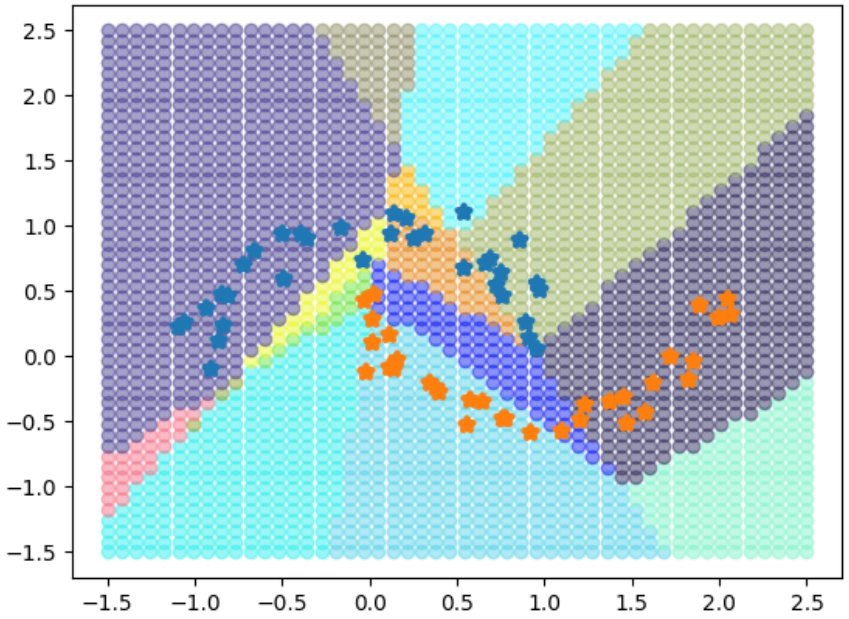
\includegraphics[width=0.8\textwidth]{include/blackbox_vs_whitebox.PNG}
    \caption{En esta gráfica de \cite{aytekin2022neural}, se muestra cómo un árbol de decisión clasifica un conjunto de datos dividiendo el espacio de características en regiones distintas, representadas por diferentes colores. Esto ilustra cómo los árboles de decisión pueden mejorar la interpretabilidad de modelos complejos, como las redes neuronales profundas, al simplificar sus decisiones en reglas comprensibles. Los puntos indican las muestras de datos, mientras que las fronteras de color reflejan los límites de decisión del modelo, facilitando la comprensión de sus predicciones.}
\end{figure}

\subsection{Confianza en Visualizaciones}

La visualización de datos juega un papel fundamental en la forma en que los usuarios interpretan y confían en los resultados de los modelos de aprendizaje automático. Estas visualizaciones pueden hacer que los modelos complejos sean más comprensibles al proporcionar una representación gráfica de los datos y las decisiones del modelo. Sin embargo, esta simplificación visual también conlleva ciertos riesgos que pueden afectar significativamente la confianza del usuario \cite{Poursabzi-2021, Kaur-2020}. 

Por un lado, las visualizaciones eficaces pueden mejorar la transparencia y facilitar la comprensión de las predicciones del modelo. Diagramas de árboles de decisión, gráficos de reglas y otros tipos de visualizaciones pueden ayudar a los usuarios a seguir el proceso de toma de decisiones de un modelo, aumentando así su confianza en la precisión y confiabilidad de las predicciones. (Véase Figura \ref{fig:confianza_visualizaciones}).

\begin{figure}[H]
    \centering
    \begin{subfigure}[b]{0.72\textwidth}
        \centering
        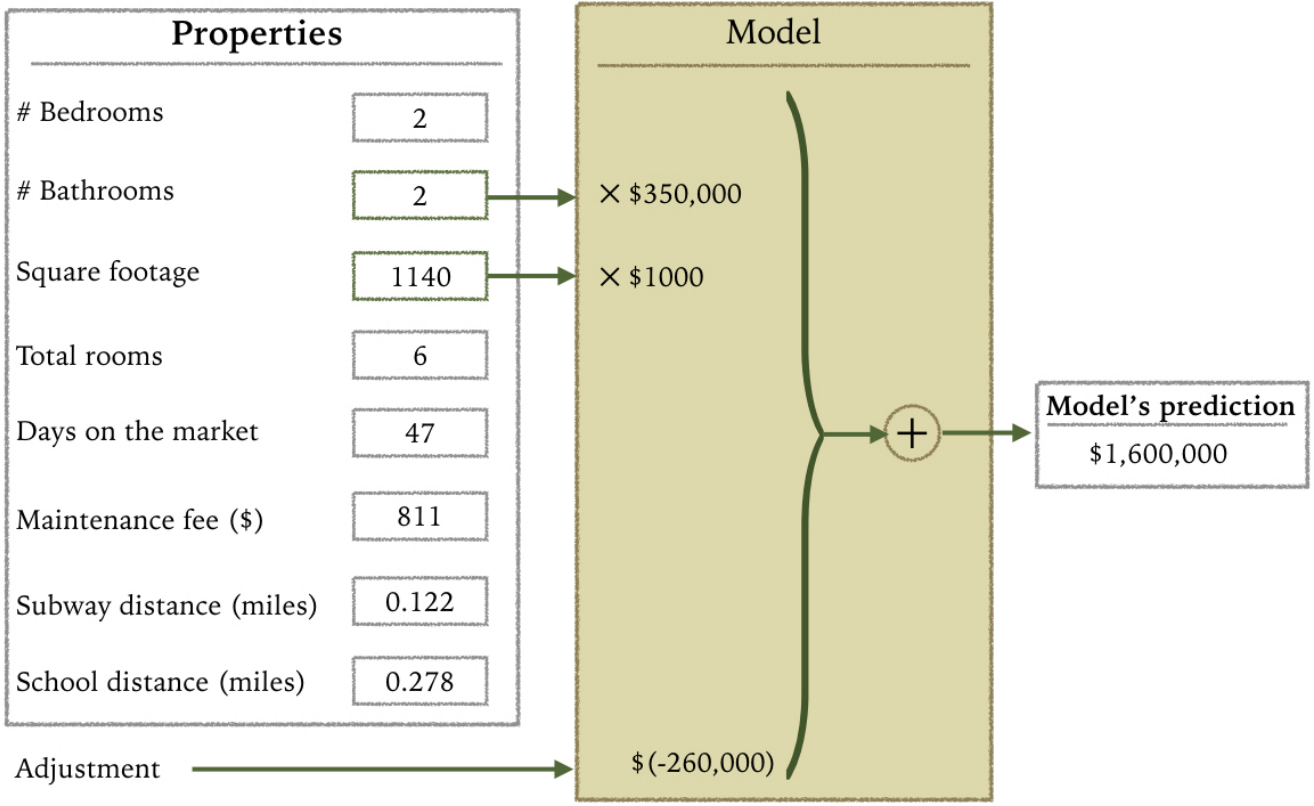
\includegraphics[width=\textwidth]{include/clear_model.PNG}
        \caption{Modelo Transparente (CLEAR-2): Muestra los cálculos internos, lo que puede aumentar la confianza del usuario, pero también sobrecargar de información.}
        \label{fig:clear_model}
    \end{subfigure}
    
    \vspace{0.5cm} % Añade un espacio vertical de 0.5 cm entre las subfiguras
    
    \begin{subfigure}[b]{0.72\textwidth}
        \centering
        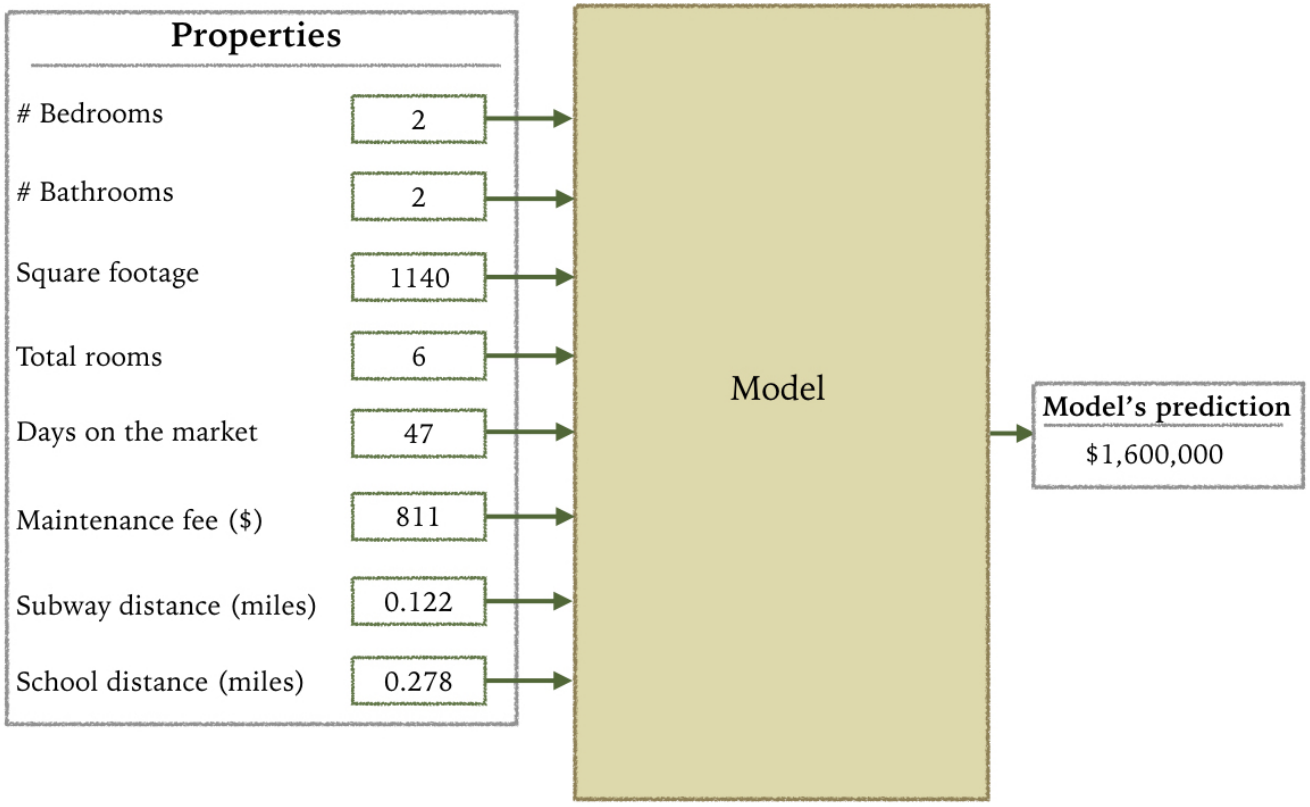
\includegraphics[width=\textwidth]{include/black_model.PNG}
        \caption{Modelo de Caja Negra (BB-8): Oculta los cálculos internos, lo que reduce la transparencia, pero evita la sobrecarga cognitiva.}
        \label{fig:black_model}
    \end{subfigure}
    \caption{Adaptación de las condiciones experimentales de Poursabzi et al. \cite{Poursabzi-2021}, que muestran cómo la presentación del modelo afecta la confianza del usuario.}
    \label{fig:confianza_visualizaciones}
\end{figure}


Por otro lado, la confianza en las visualizaciones puede llevar a una comprensión superficial o a una confianza excesiva en los resultados. Investigaciones han demostrado que los usuarios tienden a confiar más en modelos cuyos resultados están respaldados por visualizaciones atractivas, incluso si no comprenden completamente los algoritmos subyacentes \cite{Kaur-2020}. Por ejemplo, en la Figura \ref{fig:confianza_experimento}, se ilustra cómo la presentación de los resultados puede influir en la percepción de los usuarios. Este fenómeno puede llevar a que los usuarios acepten las decisiones de los modelos sin cuestionarlas o sin detectar posibles errores, simplemente porque la visualización es persuasiva. 

\begin{figure}[htbp]
    \centering
    \begin{subfigure}[b]{0.485\textwidth}
        \centering
        \fbox{
            \begin{minipage}[c][3cm][c]{\textwidth} % Ajusta 6cm a la altura deseada
                \centering
                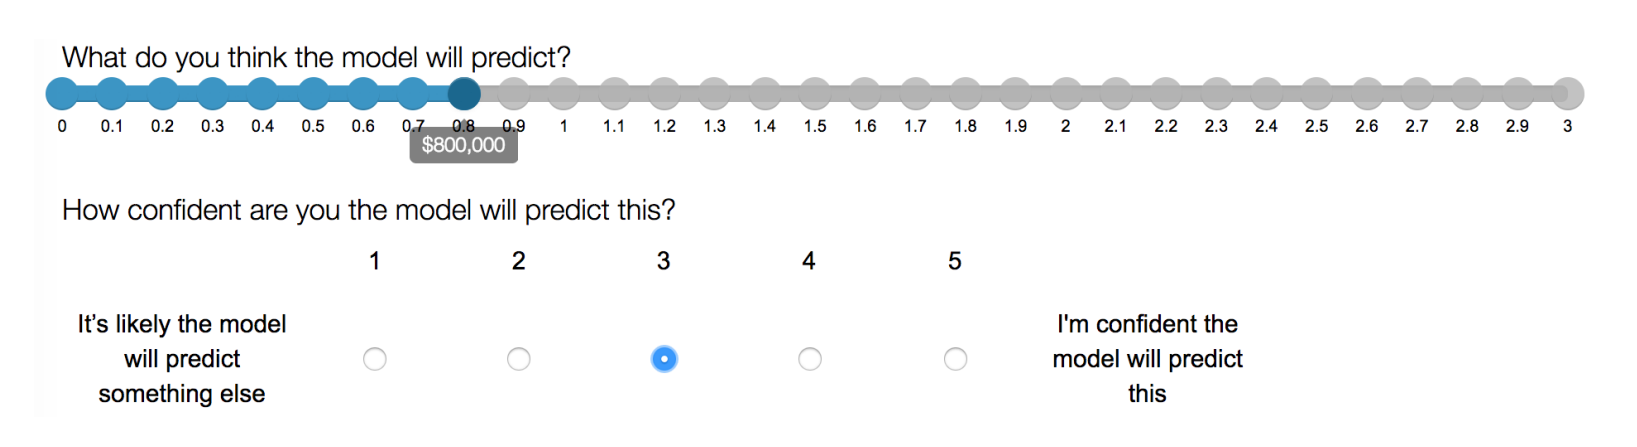
\includegraphics[width=\textwidth]{include/question1.PNG}
            \end{minipage}
        }
        \caption{Paso 1: Los participantes adivinan lo que el modelo predecirá y expresan su confianza en esa suposición.}
        \label{fig:question1}
    \end{subfigure}
    \hfill
    \begin{subfigure}[b]{0.485\textwidth}
        \centering
        \fbox{
            \begin{minipage}[c][3cm][c]{\textwidth} % Ajusta 6cm a la altura deseada
                \centering
                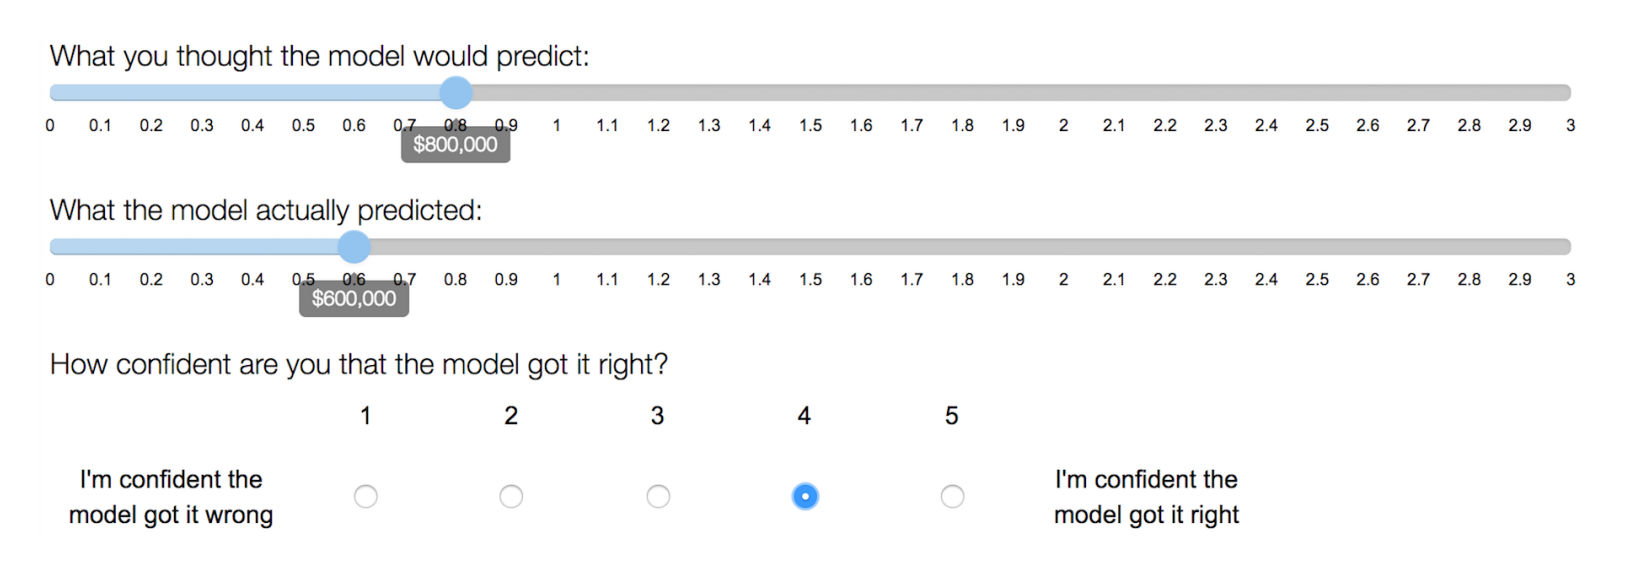
\includegraphics[width=\textwidth]{include/question2.PNG}
            \end{minipage}
        }
        \caption{Paso 2: Los participantes ajustan su confianza en la predicción del modelo después de conocer el resultado.}
        \label{fig:question2}
    \end{subfigure}
    \caption{Adaptación de las fases del experimento de Poursabzi et al. \cite{Poursabzi-2021}.}
    \label{fig:confianza_experimento}
\end{figure}

Además, las visualizaciones pueden ocultar la complejidad o ambigüedad de los datos, lo que resulta en una representación simplificada que no refleja completamente las incertidumbres o limitaciones del modelo. Como se observa en la Figura \ref{fig:experiment1_comparison}, es crucial que las visualizaciones se diseñen con cuidado para evitar inducir una falsa sensación de confianza o comprensión.

\begin{figure}[H]
    \centering
    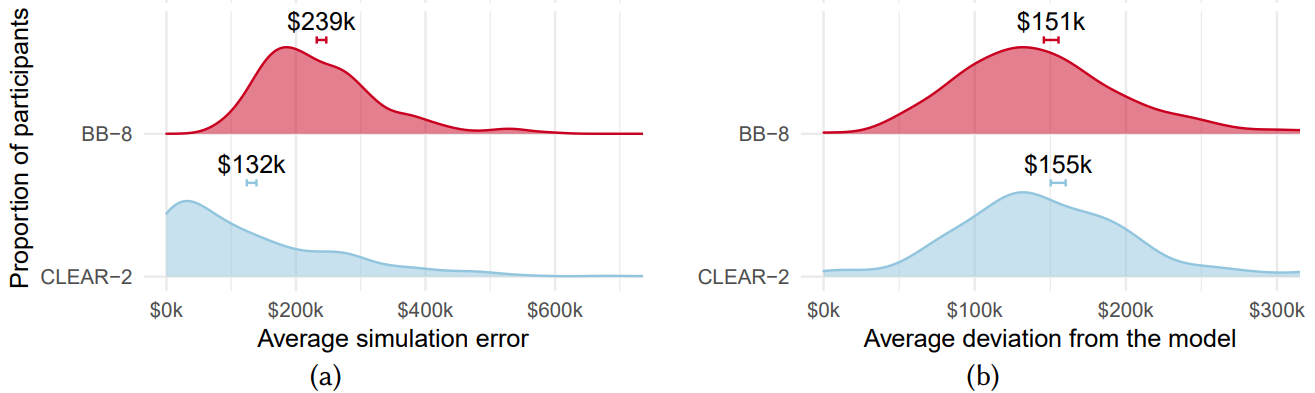
\includegraphics[width=1\textwidth]{include/error1.PNG}
    \caption{Resultados del Experimento 1 que comparan la percepción de los usuarios sobre dos tipos de modelos: un modelo de caja negra (BB-8) y un modelo transparente (CLEAR-2). En (a), se muestra el error promedio de simulación, donde los participantes tienden a percibir mayores errores en el modelo de caja negra en comparación con el modelo transparente. En (b), se presenta la desviación promedio de las predicciones del modelo respecto a los valores reales, indicando cómo los participantes evalúan la precisión del modelo según su nivel de transparencia. Adaptado de Poursabzi et al. \cite{Poursabzi-2021}.}
    \label{fig:experiment1_comparison}
\end{figure}

\section{Evaluación de la Interpretabilidad: Métodos y Métricas}

Para garantizar que los usuarios finales comprendan cómo funcionan los modelos de IA, es crucial llevar a cabo estudios empíricos que evalúen su interpretabilidad \cite{doshi2017towards}.

\subsection{Necesidad de Validación Empírica}

La interpretabilidad no es un concepto absoluto; varía según el contexto, el modelo y las expectativas de los usuarios finales \cite{lipton2016mythos}. Por ello, no se puede asumir que un modelo es interpretativo sin estudios empíricos que lo validen, los cuales permiten evaluar cómo los usuarios interactúan con los modelos, comprenden sus decisiones y cómo esta comprensión afecta su confianza y capacidad para detectar errores o sesgos \cite{Kaur-2020}.

Estos estudios también identifican las características del modelo más relevantes para los usuarios y cómo estas influyen en su toma de decisiones, proporcionando información valiosa para adaptar las explicaciones del modelo a diferentes necesidades \cite{ribeiro2016should}. Las metodologías empíricas, como experimentos con usuarios, encuestas, entrevistas o evaluación de tareas, permiten medir la capacidad de los usuarios para entender y utilizar las salidas del modelo de manera efectiva, desarrollando así herramientas adaptadas a diversos contextos \cite{doshi2017towards}.

\subsection{Métodos de Evaluación}

Existen varios métodos para evaluar la interpretabilidad de los modelos de aprendizaje automático. Algunos de los enfoques más comunes incluyen:

\begin{itemize}
    \item \textit{Estudios de Usuario:} involucran experimentos con usuarios reales para evaluar cómo entienden y perciben la interpretabilidad de un modelo. Por ejemplo, se puede medir el tiempo que los usuarios tardan en comprender una predicción o su precisión al identificar errores en las predicciones del modelo. Este tipo de estudios es particularmente útil en entornos donde la decisión basada en el modelo tiene un impacto crítico, como en diagnósticos médicos o aplicaciones financieras \cite{Kaur-2020}.
    
    \item \textit{Métricas Cuantitativas:} estas métricas miden características específicas de los modelos que se consideran proxies de interpretabilidad, tales como la simplicidad, la consistencia y la cobertura de las reglas en los modelos basados en reglas como los \textit{Interpretable Decision Sets} (IDS) y los árboles de decisión (DT) \cite{gilpin2018explaining}. Ejemplos incluyen el número de nodos en un árbol de decisión o la longitud de una regla en un conjunto de reglas. Las métricas cuantitativas permiten una evaluación objetiva de la interpretabilidad, aunque no siempre capturan completamente la percepción del usuario.
    
    \item \textit{Evaluación Basada en Tareas:} evalúa cómo los usuarios utilizan el modelo para completar tareas específicas. Por ejemplo, se podría evaluar si los usuarios pueden hacer predicciones más precisas con la ayuda del modelo interpretativo o si pueden identificar correctamente los errores cuando se les presenta una visualización del modelo. Este enfoque es útil para validar la efectividad práctica de un modelo en escenarios del mundo real \cite{doshi2017towards}.
    
    \item \textit{Encuestas y Cuestionarios:} herramientas como cuestionarios estandarizados pueden medir la percepción de los usuarios sobre la transparencia, la facilidad de comprensión y la confianza en el modelo \cite{ribeiro2016should}. Los cuestionarios pueden incluir preguntas sobre cuán claro es el modelo, cuán fácil es de entender, y cuánta confianza inspira en sus decisiones \cite{Kaur-2020}. Estas herramientas son esenciales para capturar las percepciones subjetivas de los usuarios y ajustar los modelos interpretativos a sus necesidades específicas.
\end{itemize}

Combinar estos métodos proporciona una visión más completa y precisa de la interpretabilidad de los modelos de IA, adaptada a las necesidades y expectativas de diferentes usuarios y aplicaciones. Una evaluación integral de la interpretabilidad debe tener en cuenta tanto las métricas cuantitativas como los estudios cualitativos, para capturar tanto la objetividad de las características del modelo como las percepciones subjetivas de los usuarios \cite{doshi2017towards, Kaur-2020}.

\begin{figure}[h!]
    \centering
    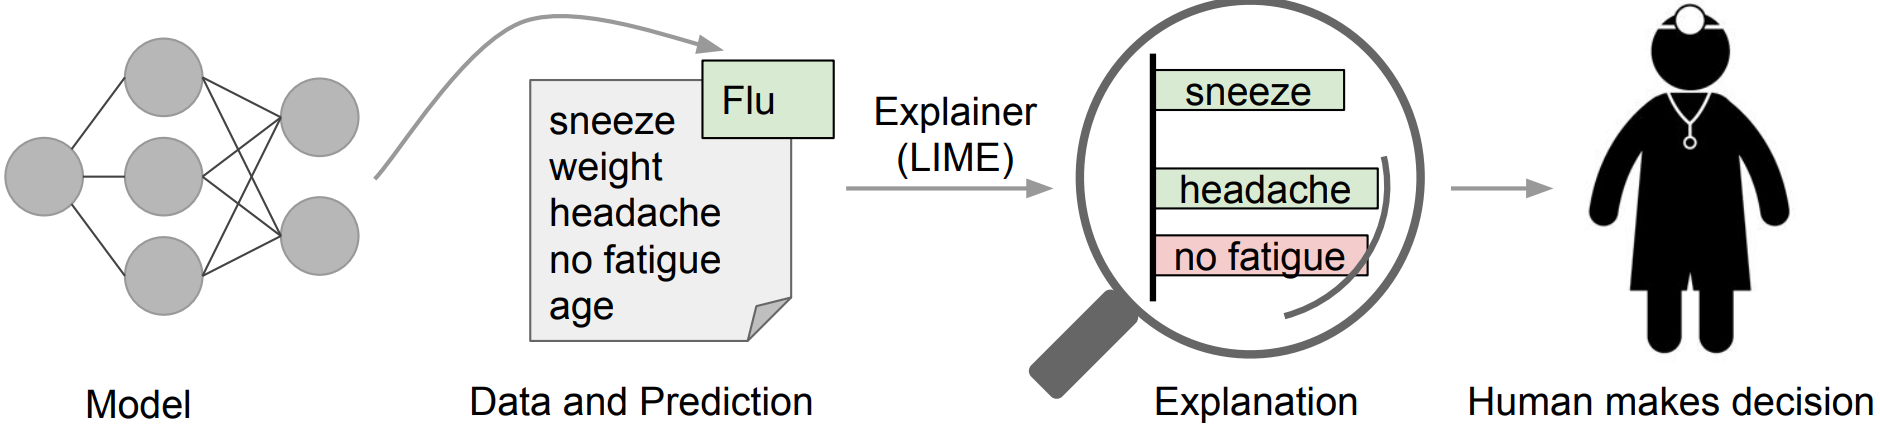
\includegraphics[width=0.7\textwidth]{include/lime.png} % Reemplaza con la ruta correcta
    \caption[Explicación de predicciones individuales usando LIME]{Explicación de predicciones individuales usando LIME. Un modelo predice que un paciente tiene gripe, y LIME resalta los síntomas en la historia del paciente que llevaron a la predicción. "Sneeze" (estornudo) y "headache" (dolor de cabeza) contribuyen a la predicción de "flu" (gripe), mientras que "no fatigue" (sin fatiga) es evidencia en contra de ella. Con esta información, un médico puede tomar una decisión informada sobre si confiar o no en la predicción del modelo.}
    \label{fig:LIME}
\end{figure}

Como se puede observar en la Figura \ref{fig:contexto_audiencia}, las diferentes herramientas de interpretabilidad, como SHAP y GAMs, ofrecen visualizaciones que varían en términos de claridad y nivel de detalle proporcionado al usuario.

\begin{figure}[h!]
    \centering
    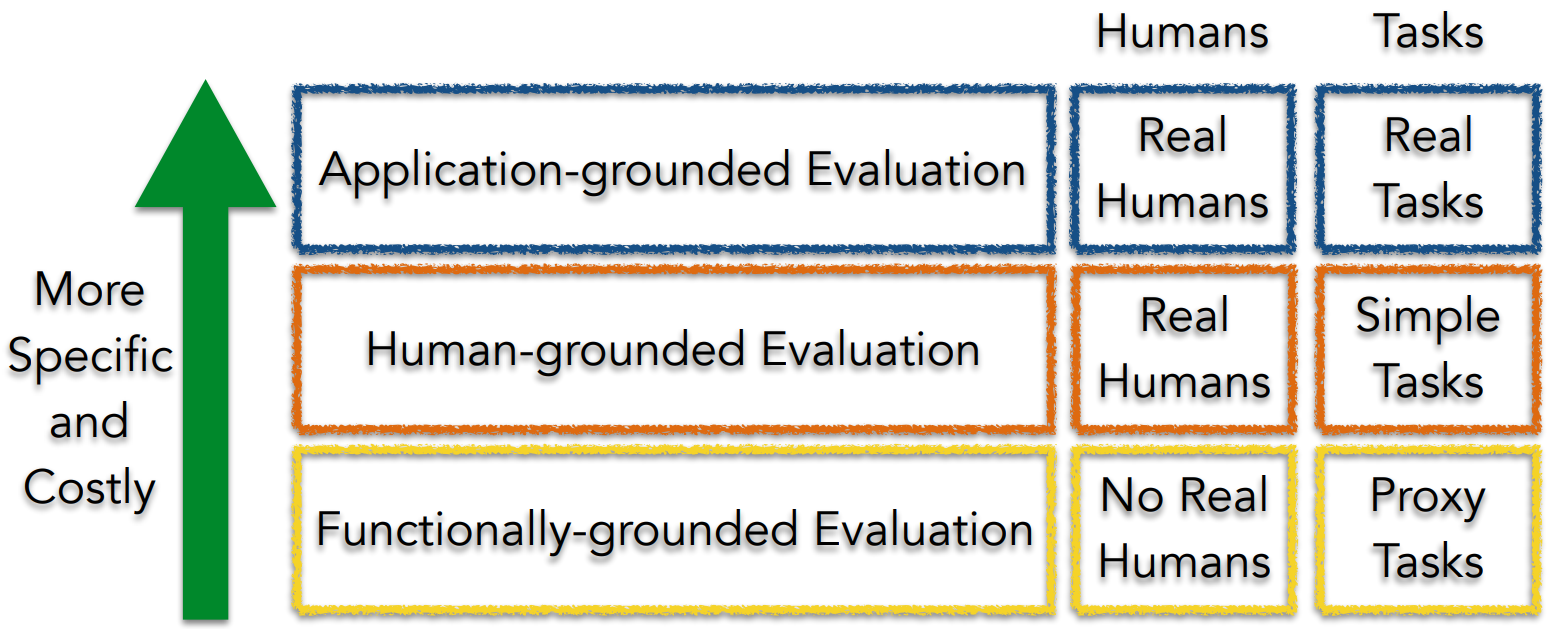
\includegraphics[width=0.7\textwidth]{include/taxonomia.PNG} % Reemplaza con la ruta correcta de la imagen
    \caption[Taxonomía de Métodos de Evaluación de Interpretabilidad]{Taxonomía de métodos de evaluación de la interpretabilidad, según Doshi-Velez y Kim (2017). La figura clasifica los métodos de evaluación en tres categorías: evaluación basada en aplicaciones, evaluación basada en humanos y evaluación basada en funciones. Cada categoría varía en términos de especificidad y costo, siendo las evaluaciones basadas en aplicaciones las más específicas y costosas, ya que implican tareas reales y usuarios humanos reales, mientras que las evaluaciones basadas en funciones son las menos costosas y específicas, al no requerir la participación de usuarios reales y emplear tareas proxy.}
    \label{fig:taxonomy_interpretability}
\end{figure}

\begin{table}[H]
    \centering
    \scriptsize % Reduce el tamaño de la fuente
    \renewcommand{\arraystretch}{1.2} % Ajusta el espaciado entre filas
    \begin{tabular}{p{3.7cm} p{2.6cm} p{2.5cm} p{1.5cm} p{3.5cm}}
        \toprule
        \textbf{Método} & \textbf{Modelo} & \textbf{Interpretabilidad} & \textbf{Usabilidad} & \textbf{Aplicación} \\
        \midrule
        Explicaciones de Saliencia & Caja Negra & Local & Media & Diagnóstico Médico \\
        Gráficos de Dependencia Parcial & Caja Blanca/Negra & Global & Alta & Análisis Económico \\
        Modelos de Reglas & Caja Blanca & Local/Global & Alta & Aplicaciones Regulatorias \\
        \bottomrule
    \end{tabular}
    \caption{Comparación simplificada de métodos de explicabilidad de modelos de aprendizaje automático. La tabla clasifica tres métodos comunes de explicabilidad: Explicaciones de Saliencia, Gráficos de Dependencia Parcial y Modelos de Reglas, según el tipo de modelo al que se aplican (caja negra o blanca), el nivel de explicabilidad que proporcionan (local o global), su usabilidad, y sus aplicaciones típicas. Esta clasificación se basa en estudios previos \cite{Kaur-2020, doshi2017towards, gilpin2018explaining} que discuten la efectividad de cada método en diferentes contextos, permitiendo seleccionar el enfoque más adecuado según las necesidades de los usuarios finales y el tipo de modelo utilizado.}
    \label{fig:comparacion_metodos_interpretabilidad}
\end{table}

\section{Resumen}

En este capítulo, se han abordado los conceptos clave relacionados con la interpretabilidad en inteligencia artificial, destacando su importancia en aplicaciones críticas donde la transparencia y la confianza en los modelos son esenciales. Se han explorado enfoques intrínsecos para mejorar la interpretabilidad, como la \textit{sparsidad}, la \textit{simulabilidad}, la \textit{modularidad} y la \textit{parsimonia}, cada uno facilitando una mejor comprensión del proceso de toma de decisiones de los modelos.

También se han examinado métodos basados en reglas, como el \textit{descubrimiento de subgrupos}, los \textit{conjuntos de contraste} y los \textit{patrones emergentes}, que identifican patrones diferenciados en los datos y proporcionan explicaciones claras de las decisiones del modelo, fundamentales para caracterizar las clases de manera comprensible para los usuarios finales.

Estos fundamentos teóricos proporcionan un marco sólido para el diseño del cuestionario de este TFM.

% ##############################################################
% ##############################################################
% ##############################################################

\chapter{Estado del Arte}

La Inteligencia Artificial Explicable (XAI, por sus siglas en inglés de \emph{eXplainable Artificial Intelligence}) se refiere a un conjunto de métodos y técnicas diseñados para hacer que los modelos de aprendizaje automático sean comprensibles e interpretables para los usuarios humanos. El objetivo es permitir a los usuarios confiar y gestionar de manera efectiva los sistemas basados en aprendizaje automático \cite{gunning2019xai}. 

En los últimos años, la comunidad científica se ha interesado en desarrollar estos métodos debido a la creciente utilización de la inteligencia artificial, lo que incrementa la necesidad de asegurar su uso ético y seguro. En este contexto, XAI se enfoca en cuatro objetivos principales \cite{curso-xai}:

\begin{itemize}
    \item \textit{Confianza y aceptación}. Para que los sistemas de IA sean ampliamente aceptados, es fundamental que los usuarios confíen en sus decisiones. Explicar cómo y por qué un modelo toma una decisión específica es crucial para construir esta confianza.
    
    \item \textit{Transparencia}. En muchas aplicaciones, especialmente en dominios sensibles como la medicina, la justicia y las finanzas, es esencial que los modelos de IA sean transparentes. Esto facilita no solo la detección y corrección de errores, sino también asegura que las decisiones sean justas y no discriminatorias.
    
    \item \textit{Cumplimiento normativo}. Diversas regulaciones, como el Reglamento General de Protección de Datos (GDPR) en Europa, exigen que las decisiones automatizadas sean explicables. Esto garantiza que los usuarios tengan derecho a una explicación clara y comprensible de cómo se toman las decisiones que les afectan.
    
    \item \textit{Mejora del modelo}. Comprender cómo funciona un modelo permite a los desarrolladores identificar áreas de mejora y ajustar los modelos para obtener mayor rendimiento y precisión.
\end{itemize}

\begin{table}[H]
    \centering
    \scriptsize % Reduce el tamaño de la fuente
    \renewcommand{\arraystretch}{1.5} % Ajusta el espaciado entre filas
    \begin{tabular}{p{3.5cm} p{5cm} p{5.8cm}}
        \toprule
        \textbf{Modelo} & \textbf{Enfoque} & \textbf{Características} \\
        \midrule
        Caja Negra & Modelos Subrogados & Uso de modelos más simples para aproximar las predicciones \\ 
        & Métricas del Efecto & Evaluación del impacto de variables (locales y globales) \\ 
        & Explicabilidad basada en Ejemplos & Uso de ejemplos específicos para explicar predicciones \\
        \midrule
        Transparentes & Intrínsecamente Interpretables & Diseñados para ser comprensibles desde su construcción \\
        & Optimización para Interpretabilidad & Ajustados específicamente para mejorar la claridad y explicación \\ 
        \bottomrule
    \end{tabular}
    \caption{Comparación de técnicas en XAI según el tipo de modelo.}
    \label{fig:cuadro-xai}
\end{table}

Los métodos y técnicas desarrollados en XAI se pueden agrupar en dos categorías principales según el tipo de modelo: modelos de caja negra y modelos transparentes \cite{curso-xai}. Estas categorías se subdividen en técnicas específicas, como se muestra en el Cuadro \ref{fig:cuadro-xai}.


\section{XAI para Modelos de Caja Negra}

Aunque este trabajo no se enfoca en métodos aplicables a modelos de caja negra, es importante mencionarlos para brindar un panorama completo de la Inteligencia Artificial Explicable (XAI). En general, un \emph{modelo de caja negra} es aquel cuyo funcionamiento interno es desconocido o no es interpretable. Esto puede deberse a que su acceso está restringido (por propiedad intelectual) o porque su mecanismo de predicción es inherentemente complejo, como en el caso de las redes neuronales \cite{curso-xai, Rudin-2019}.

Existen tres tipos principales de técnicas para abordar la explicabilidad en modelos de caja negra \cite{curso-xai}:

\begin{itemize}
    \item \textit{Modelos subrogados}: Se refiere a la creación de un modelo más sencillo e interpretable que imita las predicciones del modelo de caja negra. Este modelo subrogado puede aproximar el comportamiento del modelo original de manera \textit{local} (para un subconjunto específico de datos de entrada) o \textit{global} (para el conjunto completo de datos).
    
    \item \textit{Explicabilidad basada en ejemplos}: Busca explicar una predicción específica proporcionando ejemplos similares y contraejemplos. Esto ayuda al usuario a entender cómo diferentes características influyen en una predicción en particular.
    
    \item \textit{Métricas del efecto de las variables sobre la predicción}: Estas métricas buscan cuantificar la influencia de cada variable de entrada en las predicciones del modelo. Algunas técnicas destacadas en esta categoría son:
    \begin{itemize}
        \item \textit{LIME (Local Interpretable Model-agnostic Explanations)}: Genera explicaciones locales al identificar cuáles características influyen en una predicción específica y su efecto (positivo o negativo) \cite{ribeiro2016should}.
        \item \textit{SHAP (SHapley Additive exPlanations)}: Calcula la contribución de cada característica a la predicción utilizando conceptos de la Teoría de Juegos \cite{lundberg2017unified}.
        \item \textit{Eliminación de características}: Consiste en eliminar una característica del modelo (generalmente, reentrenando el modelo) para observar cómo cambian las predicciones sin dicha característica.
        \item \textit{Ocultamiento de características}: Similar a la eliminación, pero se ocultan parcial o totalmente algunas características, utilizado principalmente en redes neuronales convolucionales para entender qué partes de los datos son más relevantes.
    \end{itemize}
\end{itemize}


\section{XAI para Modelos Transparentes}

Los modelos transparentes son aquellos que no solo exponen el mecanismo mediante el cual generan las predicciones, sino que este proceso es fácilmente comprensible para un usuario humano. Un ejemplo clásico es la regresión lineal: es fácil entender cómo este modelo genera una predicción (mediante multiplicaciones por coeficientes y una suma), y también es fácil interpretar el significado de estos coeficientes (el valor de cada coeficiente indica el efecto de la variable correspondiente sobre la predicción).

En principio, se presume que los modelos transparentes son interpretables, es decir, que un humano puede entender el significado de los elementos del proceso de decisión y sus relaciones, como en el ejemplo de la regresión lineal. Sin embargo, en la práctica, un modelo transparente puede ser tan complejo que sobrepase la capacidad cognitiva de una persona. Por ejemplo, una regresión lineal con mil variables resulta difícil de interpretar, ya que es complejo entender el impacto de tantos factores en una predicción.

Para mejorar la interpretabilidad de estos modelos, se pueden aplicar técnicas de regularización como la \textit{Lasso}, que promueven la \textit{sparsidad} al reducir el número de variables que tienen un impacto significativo en las predicciones. Esta técnica puede observarse en la Figura \ref{fig:lasso}, donde se ilustra cómo Lasso minimiza la inclusión de variables irrelevantes, mejorando así la simplicidad y la claridad del modelo.

De esta forma, se facilita que el usuario enfoque su atención solo en las características más importantes, lo que mejora la comprensión general del modelo.






\section{Métricas de Evaluación de la Explicabilidad en Modelos Transparentes}

Esta sección discute brevemente métricas cuantitativas propuestas en la literatura para evaluar y mejorar la explicabilidad de modelos transparentes. Aunque estas métricas se justifican intuitivamente, es importante destacar que su efectividad puede depender del contexto específico del modelo y del usuario, como se ha señalado en los fundamentos teóricos (ver Figuras \ref{fig:lasso}, \ref{fig:decision_tree}, y \ref{fig:parsimonia}).

\subsection{Número de Características}

El \textit{número de características} utilizadas por un modelo es una de las métricas más comúnmente aplicadas para medir la explicabilidad \cite{Lin-2020, lakkaraju-2016, Poursabzi-2021}. Este concepto se relaciona estrechamente con la \textit{sparsidad}, ilustrada en la Figura \ref{fig:lasso}, que busca reducir el número de parámetros no nulos en un modelo para facilitar la comprensión del papel específico de cada variable en las predicciones. En modelos como las regresiones lineales (y otros modelos aditivos, como los \textit{Generalized Additive Models}), es posible promover la \textit{sparsidad} introduciendo un término de regularización en la función de pérdida, tal como se explicó en los fundamentos teóricos.

Esta idea también se extiende a otros tipos de modelos, como los árboles de decisión. Por ejemplo, \cite{Hu-2019, Lin-2020} proponen el uso de técnicas de regularización para favorecer árboles de decisión \textit{esparsos} (del inglés \textit{sparse}), utilizando programación dinámica y teoremas que garantizan un desempeño mínimo. Este enfoque promueve la simplicidad y la \textit{parsimonia}, representada en la Figura \ref{fig:parsimonia}, utilizando la menor cantidad de variables posible sin comprometer el rendimiento.

En el caso de conjuntos de decisión, \cite{lakkaraju-2016} proponen tres métricas: una para penalizar la función de pérdida basada en el número de reglas individuales en el conjunto de decisiones, otra para penalizar la longitud de las reglas, y una última para maximizar la cobertura de una regla (es decir, aplicarla al mayor número posible de datos). Este enfoque de minimización también se alinea con los principios de \textit{parsimonia} y \textit{modularidad} (ver Figura \ref{fig:parsimonia}), al reducir la complejidad del modelo mientras se mantiene la efectividad de la predicción.

\subsection{Complejidad de la Estructura del Modelo}

La \textit{complejidad de la estructura} de un modelo transparente también afecta su interpretabilidad, como se discutió en los fundamentos teóricos en relación con la \textit{simulabilidad} (ver Figura \ref{fig:decision_tree}). Diferentes configuraciones estructurales pueden hacer que un modelo sea más o menos fácil de explicar.

Por ejemplo, en los árboles de decisión, tanto el número de ramas por nodo como la profundidad del árbol influyen en su interpretabilidad. Un árbol con muchas ramas o de gran profundidad puede ser difícil de entender, contraviniendo el principio de \textit{simulabilidad} (ver Figura \ref{fig:decision_tree}), que sugiere que los modelos deben ser fáciles de reproducir y comprender por humanos. Para mitigar esto, \cite{Lin-2020} recomienda el uso de árboles binarios (cada nodo tiene solo dos ramas), y la programación dinámica para limitar la profundidad del árbol, controlando así la complejidad del modelo.

Para los conjuntos de decisión, \cite{lakkaraju-2016} sugiere el uso de listas simples de reglas, sin anidación, ya que se considera que son más fáciles de entender que las secuencias de reglas anidadas. Esta preferencia por la simplicidad y la claridad se alinea con la noción de \textit{parsimonia} (ver Figura \ref{fig:parsimonia}), donde se favorecen las soluciones más simples y directas.




\section{Métricas para la Evaluación Humana de la Interpretabilidad}

Esta sección presenta las métricas propuestas en la literatura para la evaluación humana de la interpretabilidad. Dichas métricas son esenciales para determinar si los usuarios pueden entender un modelo de aprendizaje automático, especialmente cuando se trata de modelos transparentes, como los discutidos en la Figura \ref{fig:modularidad_ebm} sobre la modularidad y en la Figura \ref{fig:decision_tree} sobre la simulabilidad. Estas métricas se dividen en dos categorías principales: cualitativas y cuantitativas, dependiendo de su enfoque para medir el entendimiento.

\subsection{Métricas cualitativas}

Las métricas cualitativas buscan evaluar la capacidad del usuario para comprender el modelo mediante la recopilación de datos no numéricos. Generalmente, estos datos se obtienen a través de entrevistas semi-estructuradas o preguntas contextualizadas \cite{Kaur-2020}. Tal como se ilustra en la Figura \ref{fig:decision_tree}, los modelos que favorecen una estructura simple, como los árboles de decisión, facilitan la comprensión del proceso de decisión por parte del usuario. En este contexto, se puede emplear una metodología en la que el usuario tenga acceso al modelo o a visualizaciones relacionadas, y un investigador formule preguntas, asigne tareas o simplemente escuche al usuario para determinar su grado de entendimiento.

Por ejemplo, \cite{Kaur-2020} realizó entrevistas semi-estructuradas para identificar las principales dificultades que enfrentan los científicos de datos al interpretar modelos complejos. Basándose en estos resultados, se diseñaron entrevistas adicionales, utilizando el mismo enfoque mostrado en la Figura \ref{fig:contexto_audiencia}, para determinar cómo los diferentes grupos de usuarios perciben la interpretabilidad de los modelos en función de su contexto y necesidades específicas.

\subsection{Métricas cuantitativas}

Las métricas cuantitativas, a diferencia de las cualitativas, se enfocan en la recopilación de datos numéricos que puedan ser analizados de manera estadística. Similar a cómo se evaluó la interpretabilidad mediante la reducción de características en la Figura \ref{fig:lasso}, estas métricas intentan medir la capacidad del usuario para comprender un modelo a través de la exactitud de sus predicciones o la eficiencia con la que completan tareas basadas en el modelo.

La métrica más común es la exactitud o el error de desviación \cite{lakkaraju-2016, Poursabzi-2021}, que consiste en solicitar al usuario que realice predicciones utilizando el modelo, como se describe en la Figura \ref{fig:modularidad_ebm}, donde los Modelos Aditivos Generalizados (GAMs) descomponen las predicciones en componentes interpretables. Esta métrica permite determinar si un usuario es capaz de seguir el razonamiento del modelo y entender cómo se llega a una predicción específica.

Adicionalmente, se emplean otras métricas como el \textit{error de simulación} \cite{Poursabzi-2021}, en las que se muestra al usuario una serie de ejemplos y se le pide realizar predicciones para evaluar su capacidad de aprendizaje sin ayuda del modelo. De manera complementaria, el uso de cuestionarios como el NASA-TLX (\emph{Task Load Index}) \cite{Hart-1988}, que puede ayudar a cuantificar la carga cognitiva que experimentan los usuarios al interactuar con el modelo, proporcionando una medida indirecta de la interpretabilidad.

En conjunto, estas métricas ofrecen una visión integral de cómo los usuarios perciben la interpretabilidad de los modelos de aprendizaje automático, conectando las técnicas teóricas presentadas en la sección de fundamentos con la evaluación práctica de la experiencia del usuario.

\section{Herramientas de Interpretabilidad para Modelos Transparentes}

A diferencia de los modelos de caja negra, que requieren explicaciones post-hoc, los modelos transparentes permiten interpretar directamente sus decisiones debido a su estructura lógica. Sin embargo, aunque estos modelos, como los árboles de decisión (DT) y los Interpretable Decision Sets (IDS), ya son comprensibles, la claridad en la presentación y las visualizaciones influyen en cómo los usuarios perciben su interpretabilidad \cite{curso-xai, Rudin-2019}. La manera en que se presentan los resultados puede facilitar o dificultar la identificación de patrones, la detección de errores y la confianza en las decisiones.

Para abordar este reto, se han desarrollado herramientas que facilitan tanto el análisis de los modelos transparentes como la exploración de cómo las visualizaciones y la estructura del modelo afectan la experiencia del usuario. Estas herramientas combinan enfoques visuales y técnicos que mejoran la comprensión y fomentan la confianza en las predicciones.

A continuación, se describen herramientas clave en el campo de la inteligencia artificial explicable que facilitan el análisis y optimización de la interpretabilidad de modelos transparentes. Estas herramientas permiten evaluar cómo la presentación visual y la estructura de un modelo influyen en la percepción de interpretabilidad y la confianza del usuario en los sistemas de IA. Además, proporcionan una base sólida para estudiar los modelos transparentes de este trabajo, aplicando metodologías prácticas y enfoques visuales que mejoran tanto la claridad como la comprensión de los modelos de decisión.

\subsection{InterpretML}

InterpretML, propuesto por \textcite{nori2019interpretml}, es un marco de código abierto diseñado para proporcionar interpretabilidad tanto en modelos de caja blanca como en técnicas de explicabilidad post-hoc para modelos de caja negra. Este marco unifica diversas técnicas y permite a los investigadores y profesionales comparar diferentes enfoques de interpretabilidad a través de una API integrada y visualizaciones interactivas.

InterpretML ofrece dos tipos principales de interpretabilidad:
\begin{itemize}
    \item Modelos de caja blanca: Estos modelos son transparentes desde su construcción, permitiendo que los usuarios comprendan directamente cómo cada característica influye en las predicciones. Ejemplos incluyen los modelos aditivos generalizados (GAM) y los modelos lineales. En la Figura \ref{fig:modularidad_ebm} se muestra un ejemplo de cómo la característica 'Edad' afecta la predicción en un modelo EBM, proporcionando una visualización clara de las relaciones entre características y resultados.
    \item Explicabilidad para modelos de caja negra: Utilizando técnicas post-hoc como dependencia parcial, LIME y SHAP, InterpretML proporciona interpretaciones locales y globales de modelos más complejos, sin necesidad de conocer su estructura interna. La Figura \ref{fig:contexto_audiencia} compara visualizaciones generadas por GAM (arriba) y SHAP (abajo), mostrando cómo diferentes enfoques interpretativos pueden ajustarse a audiencias y contextos específicos.
\end{itemize}

Una de las contribuciones clave de InterpretML es el Explainable Boosting Machine (EBM), un modelo de caja blanca basado en un modelo aditivo generalizado (GAM) que utiliza técnicas modernas como bagging y boosting para ajustar cada característica iterativamente, reduciendo la correlación entre ellas. Esto permite que el EBM logre niveles de precisión comparables a los de modelos de caja negra como los bosques aleatorios o XGBoost, pero manteniendo la interpretabilidad total.

\begin{figure}[H]
    \centering
    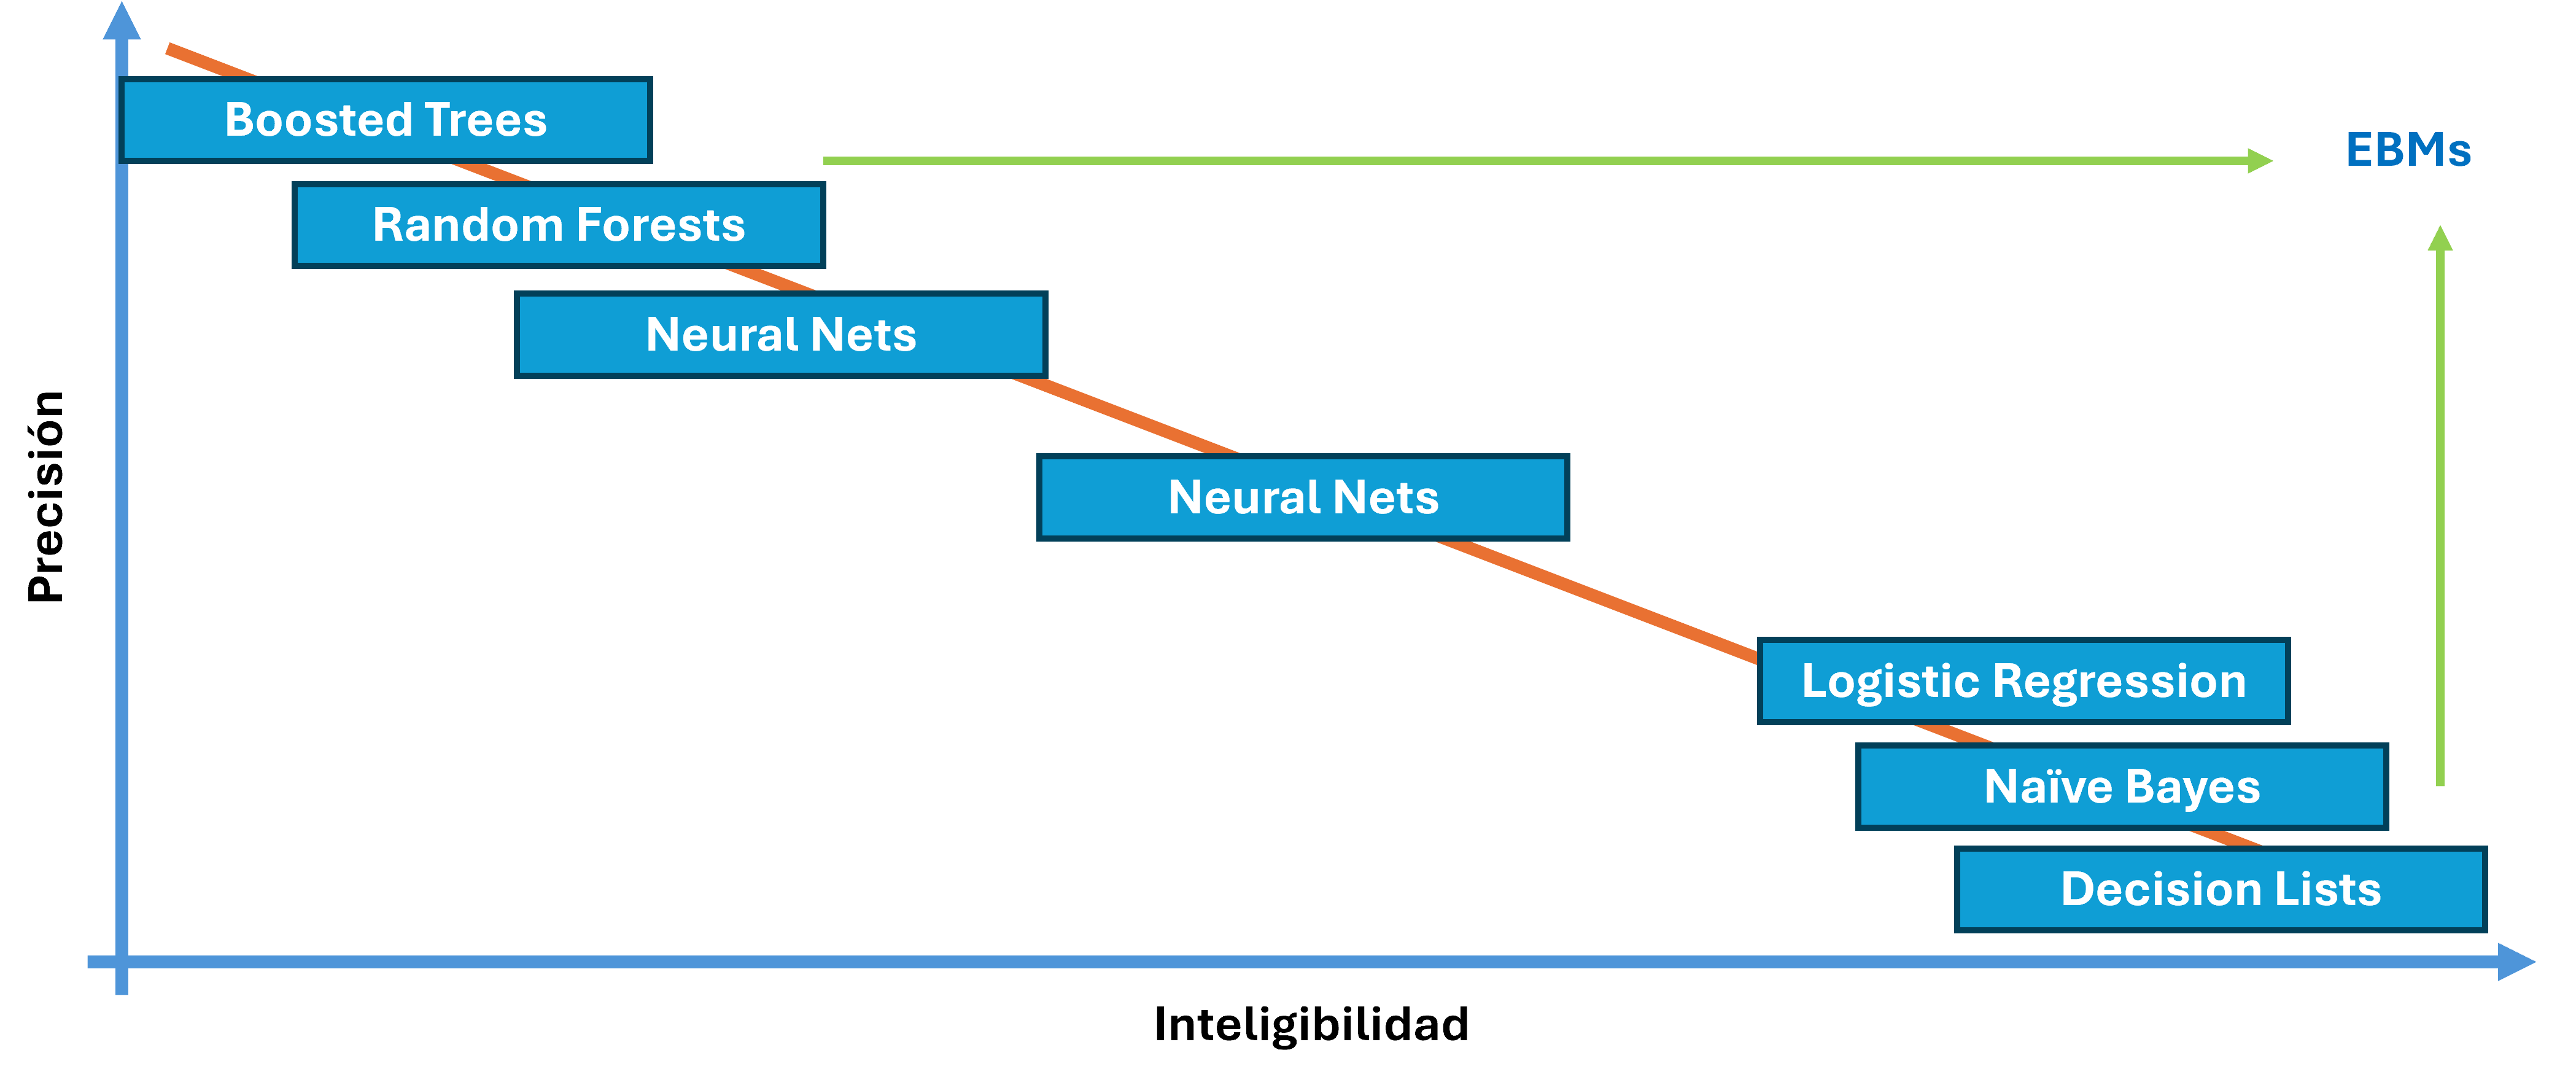
\includegraphics[width=0.9\textwidth]{include/EBMs.png}
    \caption{Gráfico comparativo de precisión e inteligibilidad de modelos de aprendizaje automático, inspirado en un gráfico presentado por \cite{microsoftEBMvideo}.}
    \label{fig:EBMs}
\end{figure}

El EBM es modular y permite visualizar cómo cada característica influye en las predicciones, facilitando la comprensión para los usuarios mediante gráficos claros, como los mostrados en la Figura \ref{fig:modularidad_ebm}, que ilustran la descomposición de una predicción individual y cómo cada característica contribuye de forma independiente.

InterpretML presenta varias ventajas:
\begin{itemize}
    \item Facilidad de comparación: La API unificada facilita la comparación de diferentes algoritmos de interpretabilidad, con integración sencilla a frameworks como scikit-learn.
    \item Interoperabilidad: Es compatible con herramientas como Jupyter Notebook y plotly, permitiendo una interacción intuitiva con los modelos y sus explicaciones.
    \item Visualización interactiva: InterpretML ofrece un panel de control interactivo que permite explorar visualmente las explicaciones generadas, ayudando a los usuarios a entender fácilmente las contribuciones de cada característica.
\end{itemize}

InterpretML ha demostrado ser útil en áreas como la salud, las finanzas y la justicia, donde la interpretabilidad es crítica. Su capacidad para combinar precisión y transparencia lo convierte en una herramienta esencial en sistemas de alta responsabilidad.

\subsection{Yellowbrick}

Yellowbrick es una biblioteca de visualización diseñada para facilitar la evaluación e interpretación de modelos de aprendizaje automático creados con scikit-learn. Esta herramienta ofrece una amplia gama de visualizaciones que permiten a los usuarios entender mejor el comportamiento de los modelos, ayudando en la toma de decisiones y mejorando la interpretabilidad de los mismos \cite{bengfort_yellowbrick_2018}.

Yellowbrick se enfoca en generar gráficos que muestran cómo las características y el rendimiento de los modelos afectan los resultados, lo cual es esencial para modelos transparentes como los DT y los IDs utilizados en este trabajo. Entre sus funcionalidades más destacadas se incluyen:

\begin{itemize}
    \item \textit{Visualización de la importancia de características}: Yellowbrick permite visualizar gráficamente la importancia relativa de las características dentro de un modelo. En el contexto de este TFM, esta funcionalidad es crucial para entender cómo las distintas características influyen en las predicciones de los modelos de decisión.
    
    \item \textit{Curvas de validación y curvas de aprendizaje}: Estas curvas permiten observar cómo el rendimiento del modelo varía según los valores de los hiperparámetros y cómo mejora a medida que recibe más datos de entrenamiento. Este tipo de visualización es útil para diagnosticar problemas de sobreajuste o subajuste, que impactan directamente en la interpretabilidad del modelo.

    \item \textit{Matrices de confusión y reportes de clasificación}: Facilitan la visualización de la matriz de confusión, mostrando cómo el modelo clasifica correctamente e incorrectamente las instancias, lo que ayuda a comprender mejor cómo cada clase es manejada por el modelo. Esta herramienta es valiosa para modelos como Árboles de Decisión, ya que proporciona un análisis visual detallado de los resultados.

    \item \textit{Curvas ROC y AUC}: Permiten evaluar el rendimiento de los modelos de clasificación, mostrando el compromiso entre la tasa de verdaderos positivos y la tasa de falsos positivos en diferentes umbrales de decisión. Estas curvas son especialmente útiles para evaluar la interpretabilidad de los modelos en términos de su capacidad para manejar errores en la clasificación.
\end{itemize}

Yellowbrick ofrece ventajas significativas, entre las que destaca su integración perfecta con scikit-learn, lo que permite a los usuarios generar visualizaciones sin una configuración adicional compleja. Además, proporciona una interfaz fácil de usar que se adapta tanto a principiantes como a expertos, facilitando la evaluación visual de los modelos de manera clara y concisa.



\subsection{Anchors}
Diseñada para generar reglas locales y fáciles de entender que explican de manera intuitiva las predicciones de un modelo. Este enfoque es ideal para modelos basados en reglas, como los IDS, ya que ofrece una explicación clara basada en ``anclas'' que describen el comportamiento de un modelo en una determinada predicción \cite{ribeiro2018anchors}.

\subsection{DiCE}
Una herramienta que genera explicaciones contrafactuales, ayudando a los usuarios a entender cómo pequeños cambios en las características de entrada podrían alterar la predicción. Aunque los modelos transparentes suelen ser interpretables, DiCE añade una capa de explicabilidad al permitir que los usuarios visualicen posibles escenarios alternativos para mejorar la comprensión de las decisiones del modelo \cite{arya2019one}.

\section{Resumen}

En este capítulo, se ha presentado una revisión de los enfoques y técnicas en Inteligencia Artificial Explicable (XAI), centrándose tanto en modelos de caja negra como en modelos transparentes. Se han discutido métodos para mejorar la interpretabilidad de los modelos de caja negra, como los modelos subrogados, la explicabilidad mediante ejemplos y las métricas del efecto de variables, resaltando cómo estos enfoques buscan hacer más comprensibles los modelos complejos cuyo funcionamiento interno no es directamente accesible.

El capítulo también ha explorado estrategias específicas para optimizar la explicabilidad en modelos transparentes, como los Árboles de Decisión (DT) y los Interpretable Decision Sets (IDS). Se han analizado técnicas como la regularización LASSO para promover la \textit{sparsidad} y la simplificación estructural, que son esenciales para mejorar la claridad y comprensión de estos modelos.

Además, se han presentado métricas cualitativas y cuantitativas para la evaluación de la interpretabilidad desde la perspectiva del usuario, proporcionando un marco para medir cómo los usuarios entienden y perciben los modelos de IA. Estas métricas, que incluyen la complejidad estructural del modelo y la capacidad de los usuarios para realizar predicciones basadas en él, permiten una evaluación integral del impacto de diferentes enfoques en la interpretabilidad, vinculando los fundamentos teóricos con su aplicación práctica.

Esta revisión proporciona la base teórica y práctica necesaria para el desarrollo del cuestionario de evaluación de interpretabilidad propuesto en este trabajo, identificando las técnicas y métricas más relevantes para alcanzar los objetivos de investigación planteados y fortalecer la comprensión de los usuarios sobre los modelos utilizados.

\chapter{Estado del Arte}

La Inteligencia Artificial Explicable (XAI, por sus siglas en inglés de \emph{eXplainable Artificial Intelligence}) se refiere a un conjunto de métodos y técnicas diseñados para hacer que los modelos de aprendizaje automático sean comprensibles e interpretables para los usuarios humanos. El objetivo es permitir a los usuarios confiar y gestionar de manera efectiva los sistemas basados en aprendizaje automático \cite{gunning2019xai}. 

En los últimos años, la comunidad científica se ha interesado en desarrollar estos métodos debido a la creciente utilización de la inteligencia artificial, lo que incrementa la necesidad de asegurar su uso ético y seguro. En este contexto, XAI se enfoca en cuatro objetivos principales \cite{curso-xai}:

\begin{itemize}
    \item \textit{Confianza y aceptación}. Para que los sistemas de IA sean ampliamente aceptados, es fundamental que los usuarios confíen en sus decisiones. Explicar cómo y por qué un modelo toma una decisión específica es crucial para construir esta confianza.
    
    \item \textit{Transparencia}. En muchas aplicaciones, especialmente en dominios sensibles como la medicina, la justicia y las finanzas, es esencial que los modelos de IA sean transparentes. Esto facilita no solo la detección y corrección de errores, sino también asegura que las decisiones sean justas y no discriminatorias.
    
    \item \textit{Cumplimiento normativo}. Diversas regulaciones, como el Reglamento General de Protección de Datos (GDPR) en Europa, exigen que las decisiones automatizadas sean explicables. Esto garantiza que los usuarios tengan derecho a una explicación clara y comprensible de cómo se toman las decisiones que les afectan.
    
    \item \textit{Mejora del modelo}. Comprender cómo funciona un modelo permite a los desarrolladores identificar áreas de mejora y ajustar los modelos para obtener mayor rendimiento y precisión.
\end{itemize}

\begin{table}[H]
    \centering
    \scriptsize % Reduce el tamaño de la fuente
    \renewcommand{\arraystretch}{1.5} % Ajusta el espaciado entre filas
    \begin{tabular}{p{3.5cm} p{5cm} p{5.8cm}}
        \toprule
        \textbf{Modelo} & \textbf{Enfoque} & \textbf{Características} \\
        \midrule
        Caja Negra & Modelos Subrogados & Uso de modelos más simples para aproximar las predicciones \\ 
        & Métricas del Efecto & Evaluación del impacto de variables (locales y globales) \\ 
        & Explicabilidad basada en Ejemplos & Uso de ejemplos específicos para explicar predicciones \\
        \midrule
        Transparentes & Intrínsecamente Interpretables & Diseñados para ser comprensibles desde su construcción \\
        & Optimización para Interpretabilidad & Ajustados específicamente para mejorar la claridad y explicación \\ 
        \bottomrule
    \end{tabular}
    \caption{Comparación de técnicas en XAI según el tipo de modelo.}
    \label{fig:cuadro-xai}
\end{table}

Los métodos y técnicas desarrollados en XAI se pueden agrupar en dos categorías principales según el tipo de modelo: modelos de caja negra y modelos transparentes \cite{curso-xai}. Estas categorías se subdividen en técnicas específicas, como se muestra en el Cuadro \ref{fig:cuadro-xai}.


\section{XAI para Modelos de Caja Negra}

Aunque este trabajo no se enfoca en métodos aplicables a modelos de caja negra, es importante mencionarlos para brindar un panorama completo de la Inteligencia Artificial Explicable (XAI). En general, un \emph{modelo de caja negra} es aquel cuyo funcionamiento interno es desconocido o no es interpretable. Esto puede deberse a que su acceso está restringido (por propiedad intelectual) o porque su mecanismo de predicción es inherentemente complejo, como en el caso de las redes neuronales \cite{curso-xai, Rudin-2019}.

Existen tres tipos principales de técnicas para abordar la explicabilidad en modelos de caja negra \cite{curso-xai}:

\begin{itemize}
    \item \textit{Modelos subrogados}: Se refiere a la creación de un modelo más sencillo e interpretable que imita las predicciones del modelo de caja negra. Este modelo subrogado puede aproximar el comportamiento del modelo original de manera \textit{local} (para un subconjunto específico de datos de entrada) o \textit{global} (para el conjunto completo de datos).
    
    \item \textit{Explicabilidad basada en ejemplos}: Busca explicar una predicción específica proporcionando ejemplos similares y contraejemplos. Esto ayuda al usuario a entender cómo diferentes características influyen en una predicción en particular.
    
    \item \textit{Métricas del efecto de las variables sobre la predicción}: Estas métricas buscan cuantificar la influencia de cada variable de entrada en las predicciones del modelo. Algunas técnicas destacadas en esta categoría son:
    \begin{itemize}
        \item \textit{LIME (Local Interpretable Model-agnostic Explanations)}: Genera explicaciones locales al identificar cuáles características influyen en una predicción específica y su efecto (positivo o negativo) \cite{ribeiro2016should}.
        \item \textit{SHAP (SHapley Additive exPlanations)}: Calcula la contribución de cada característica a la predicción utilizando conceptos de la Teoría de Juegos \cite{lundberg2017unified}.
        \item \textit{Eliminación de características}: Consiste en eliminar una característica del modelo (generalmente, reentrenando el modelo) para observar cómo cambian las predicciones sin dicha característica.
        \item \textit{Ocultamiento de características}: Similar a la eliminación, pero se ocultan parcial o totalmente algunas características, utilizado principalmente en redes neuronales convolucionales para entender qué partes de los datos son más relevantes.
    \end{itemize}
\end{itemize}


\section{XAI para Modelos Transparentes}

Los modelos transparentes son aquellos que no solo exponen el mecanismo mediante el cual generan las predicciones, sino que este proceso es fácilmente comprensible para un usuario humano. Un ejemplo clásico es la regresión lineal: es fácil entender cómo este modelo genera una predicción (mediante multiplicaciones por coeficientes y una suma), y también es fácil interpretar el significado de estos coeficientes (el valor de cada coeficiente indica el efecto de la variable correspondiente sobre la predicción).

En principio, se presume que los modelos transparentes son interpretables, es decir, que un humano puede entender el significado de los elementos del proceso de decisión y sus relaciones, como en el ejemplo de la regresión lineal. Sin embargo, en la práctica, un modelo transparente puede ser tan complejo que sobrepase la capacidad cognitiva de una persona. Por ejemplo, una regresión lineal con mil variables resulta difícil de interpretar, ya que es complejo entender el impacto de tantos factores en una predicción.

Para mejorar la interpretabilidad de estos modelos, se pueden aplicar técnicas de regularización como la \textit{Lasso}, que promueven la \textit{sparsidad} al reducir el número de variables que tienen un impacto significativo en las predicciones. Esta técnica puede observarse en la Figura \ref{fig:lasso}, donde se ilustra cómo Lasso minimiza la inclusión de variables irrelevantes, mejorando así la simplicidad y la claridad del modelo.

De esta forma, se facilita que el usuario enfoque su atención solo en las características más importantes, lo que mejora la comprensión general del modelo.






\section{Métricas de Evaluación de la Explicabilidad en Modelos Transparentes}

Esta sección discute brevemente métricas cuantitativas propuestas en la literatura para evaluar y mejorar la explicabilidad de modelos transparentes. Aunque estas métricas se justifican intuitivamente, es importante destacar que su efectividad puede depender del contexto específico del modelo y del usuario, como se ha señalado en los fundamentos teóricos (ver Figuras \ref{fig:lasso}, \ref{fig:decision_tree}, y \ref{fig:parsimonia}).

\subsection{Número de Características}

El \textit{número de características} utilizadas por un modelo es una de las métricas más comúnmente aplicadas para medir la explicabilidad \cite{Lin-2020, lakkaraju-2016, Poursabzi-2021}. Este concepto se relaciona estrechamente con la \textit{sparsidad}, ilustrada en la Figura \ref{fig:lasso}, que busca reducir el número de parámetros no nulos en un modelo para facilitar la comprensión del papel específico de cada variable en las predicciones. En modelos como las regresiones lineales (y otros modelos aditivos, como los \textit{Generalized Additive Models}), es posible promover la \textit{sparsidad} introduciendo un término de regularización en la función de pérdida, tal como se explicó en los fundamentos teóricos.

Esta idea también se extiende a otros tipos de modelos, como los árboles de decisión. Por ejemplo, \cite{Hu-2019, Lin-2020} proponen el uso de técnicas de regularización para favorecer árboles de decisión \textit{esparsos} (del inglés \textit{sparse}), utilizando programación dinámica y teoremas que garantizan un desempeño mínimo. Este enfoque promueve la simplicidad y la \textit{parsimonia}, representada en la Figura \ref{fig:parsimonia}, utilizando la menor cantidad de variables posible sin comprometer el rendimiento.

En el caso de conjuntos de decisión, \cite{lakkaraju-2016} proponen tres métricas: una para penalizar la función de pérdida basada en el número de reglas individuales en el conjunto de decisiones, otra para penalizar la longitud de las reglas, y una última para maximizar la cobertura de una regla (es decir, aplicarla al mayor número posible de datos). Este enfoque de minimización también se alinea con los principios de \textit{parsimonia} y \textit{modularidad} (ver Figura \ref{fig:parsimonia}), al reducir la complejidad del modelo mientras se mantiene la efectividad de la predicción.

\subsection{Complejidad de la Estructura del Modelo}

La \textit{complejidad de la estructura} de un modelo transparente también afecta su interpretabilidad, como se discutió en los fundamentos teóricos en relación con la \textit{simulabilidad} (ver Figura \ref{fig:decision_tree}). Diferentes configuraciones estructurales pueden hacer que un modelo sea más o menos fácil de explicar.

Por ejemplo, en los árboles de decisión, tanto el número de ramas por nodo como la profundidad del árbol influyen en su interpretabilidad. Un árbol con muchas ramas o de gran profundidad puede ser difícil de entender, contraviniendo el principio de \textit{simulabilidad} (ver Figura \ref{fig:decision_tree}), que sugiere que los modelos deben ser fáciles de reproducir y comprender por humanos. Para mitigar esto, \cite{Lin-2020} recomienda el uso de árboles binarios (cada nodo tiene solo dos ramas), y la programación dinámica para limitar la profundidad del árbol, controlando así la complejidad del modelo.

Para los conjuntos de decisión, \cite{lakkaraju-2016} sugiere el uso de listas simples de reglas, sin anidación, ya que se considera que son más fáciles de entender que las secuencias de reglas anidadas. Esta preferencia por la simplicidad y la claridad se alinea con la noción de \textit{parsimonia} (ver Figura \ref{fig:parsimonia}), donde se favorecen las soluciones más simples y directas.




\section{Métricas para la Evaluación Humana de la Interpretabilidad}

Esta sección presenta las métricas propuestas en la literatura para la evaluación humana de la interpretabilidad. Dichas métricas son esenciales para determinar si los usuarios pueden entender un modelo de aprendizaje automático, especialmente cuando se trata de modelos transparentes, como los discutidos en la Figura \ref{fig:modularidad_ebm} sobre la modularidad y en la Figura \ref{fig:decision_tree} sobre la simulabilidad. Estas métricas se dividen en dos categorías principales: cualitativas y cuantitativas, dependiendo de su enfoque para medir el entendimiento.

\subsection{Métricas cualitativas}

Las métricas cualitativas buscan evaluar la capacidad del usuario para comprender el modelo mediante la recopilación de datos no numéricos. Generalmente, estos datos se obtienen a través de entrevistas semi-estructuradas o preguntas contextualizadas \cite{Kaur-2020}. Tal como se ilustra en la Figura \ref{fig:decision_tree}, los modelos que favorecen una estructura simple, como los árboles de decisión, facilitan la comprensión del proceso de decisión por parte del usuario. En este contexto, se puede emplear una metodología en la que el usuario tenga acceso al modelo o a visualizaciones relacionadas, y un investigador formule preguntas, asigne tareas o simplemente escuche al usuario para determinar su grado de entendimiento.

Por ejemplo, \cite{Kaur-2020} realizó entrevistas semi-estructuradas para identificar las principales dificultades que enfrentan los científicos de datos al interpretar modelos complejos. Basándose en estos resultados, se diseñaron entrevistas adicionales, utilizando el mismo enfoque mostrado en la Figura \ref{fig:contexto_audiencia}, para determinar cómo los diferentes grupos de usuarios perciben la interpretabilidad de los modelos en función de su contexto y necesidades específicas.

\subsection{Métricas cuantitativas}

Las métricas cuantitativas, a diferencia de las cualitativas, se enfocan en la recopilación de datos numéricos que puedan ser analizados de manera estadística. Similar a cómo se evaluó la interpretabilidad mediante la reducción de características en la Figura \ref{fig:lasso}, estas métricas intentan medir la capacidad del usuario para comprender un modelo a través de la exactitud de sus predicciones o la eficiencia con la que completan tareas basadas en el modelo.

La métrica más común es la exactitud o el error de desviación \cite{lakkaraju-2016, Poursabzi-2021}, que consiste en solicitar al usuario que realice predicciones utilizando el modelo, como se describe en la Figura \ref{fig:modularidad_ebm}, donde los Modelos Aditivos Generalizados (GAMs) descomponen las predicciones en componentes interpretables. Esta métrica permite determinar si un usuario es capaz de seguir el razonamiento del modelo y entender cómo se llega a una predicción específica.

Adicionalmente, se emplean otras métricas como el \textit{error de simulación} \cite{Poursabzi-2021}, en las que se muestra al usuario una serie de ejemplos y se le pide realizar predicciones para evaluar su capacidad de aprendizaje sin ayuda del modelo. De manera complementaria, el uso de cuestionarios como el NASA-TLX (\emph{Task Load Index}) \cite{Hart-1988}, que puede ayudar a cuantificar la carga cognitiva que experimentan los usuarios al interactuar con el modelo, proporcionando una medida indirecta de la interpretabilidad.

En conjunto, estas métricas ofrecen una visión integral de cómo los usuarios perciben la interpretabilidad de los modelos de aprendizaje automático, conectando las técnicas teóricas presentadas en la sección de fundamentos con la evaluación práctica de la experiencia del usuario.

\section{Herramientas de Interpretabilidad para Modelos Transparentes}

A diferencia de los modelos de caja negra, que requieren explicaciones post-hoc, los modelos transparentes permiten interpretar directamente sus decisiones debido a su estructura lógica. Sin embargo, aunque estos modelos, como los árboles de decisión (DT) y los Interpretable Decision Sets (IDS), ya son comprensibles, la claridad en la presentación y las visualizaciones influyen en cómo los usuarios perciben su interpretabilidad \cite{curso-xai, Rudin-2019}. La manera en que se presentan los resultados puede facilitar o dificultar la identificación de patrones, la detección de errores y la confianza en las decisiones.

Para abordar este reto, se han desarrollado herramientas que facilitan tanto el análisis de los modelos transparentes como la exploración de cómo las visualizaciones y la estructura del modelo afectan la experiencia del usuario. Estas herramientas combinan enfoques visuales y técnicos que mejoran la comprensión y fomentan la confianza en las predicciones.

A continuación, se describen herramientas clave en el campo de la inteligencia artificial explicable que facilitan el análisis y optimización de la interpretabilidad de modelos transparentes. Estas herramientas permiten evaluar cómo la presentación visual y la estructura de un modelo influyen en la percepción de interpretabilidad y la confianza del usuario en los sistemas de IA. Además, proporcionan una base sólida para estudiar los modelos transparentes de este trabajo, aplicando metodologías prácticas y enfoques visuales que mejoran tanto la claridad como la comprensión de los modelos de decisión.

\subsection{InterpretML}

InterpretML, propuesto por \textcite{nori2019interpretml}, es un marco de código abierto diseñado para proporcionar interpretabilidad tanto en modelos de caja blanca como en técnicas de explicabilidad post-hoc para modelos de caja negra. Este marco unifica diversas técnicas y permite a los investigadores y profesionales comparar diferentes enfoques de interpretabilidad a través de una API integrada y visualizaciones interactivas.

InterpretML ofrece dos tipos principales de interpretabilidad:
\begin{itemize}
    \item Modelos de caja blanca: Estos modelos son transparentes desde su construcción, permitiendo que los usuarios comprendan directamente cómo cada característica influye en las predicciones. Ejemplos incluyen los modelos aditivos generalizados (GAM) y los modelos lineales. En la Figura \ref{fig:modularidad_ebm} se muestra un ejemplo de cómo la característica 'Edad' afecta la predicción en un modelo EBM, proporcionando una visualización clara de las relaciones entre características y resultados.
    \item Explicabilidad para modelos de caja negra: Utilizando técnicas post-hoc como dependencia parcial, LIME y SHAP, InterpretML proporciona interpretaciones locales y globales de modelos más complejos, sin necesidad de conocer su estructura interna. La Figura \ref{fig:contexto_audiencia} compara visualizaciones generadas por GAM (arriba) y SHAP (abajo), mostrando cómo diferentes enfoques interpretativos pueden ajustarse a audiencias y contextos específicos.
\end{itemize}

Una de las contribuciones clave de InterpretML es el Explainable Boosting Machine (EBM), un modelo de caja blanca basado en un modelo aditivo generalizado (GAM) que utiliza técnicas modernas como bagging y boosting para ajustar cada característica iterativamente, reduciendo la correlación entre ellas. Esto permite que el EBM logre niveles de precisión comparables a los de modelos de caja negra como los bosques aleatorios o XGBoost, pero manteniendo la interpretabilidad total.

\begin{figure}[H]
    \centering
    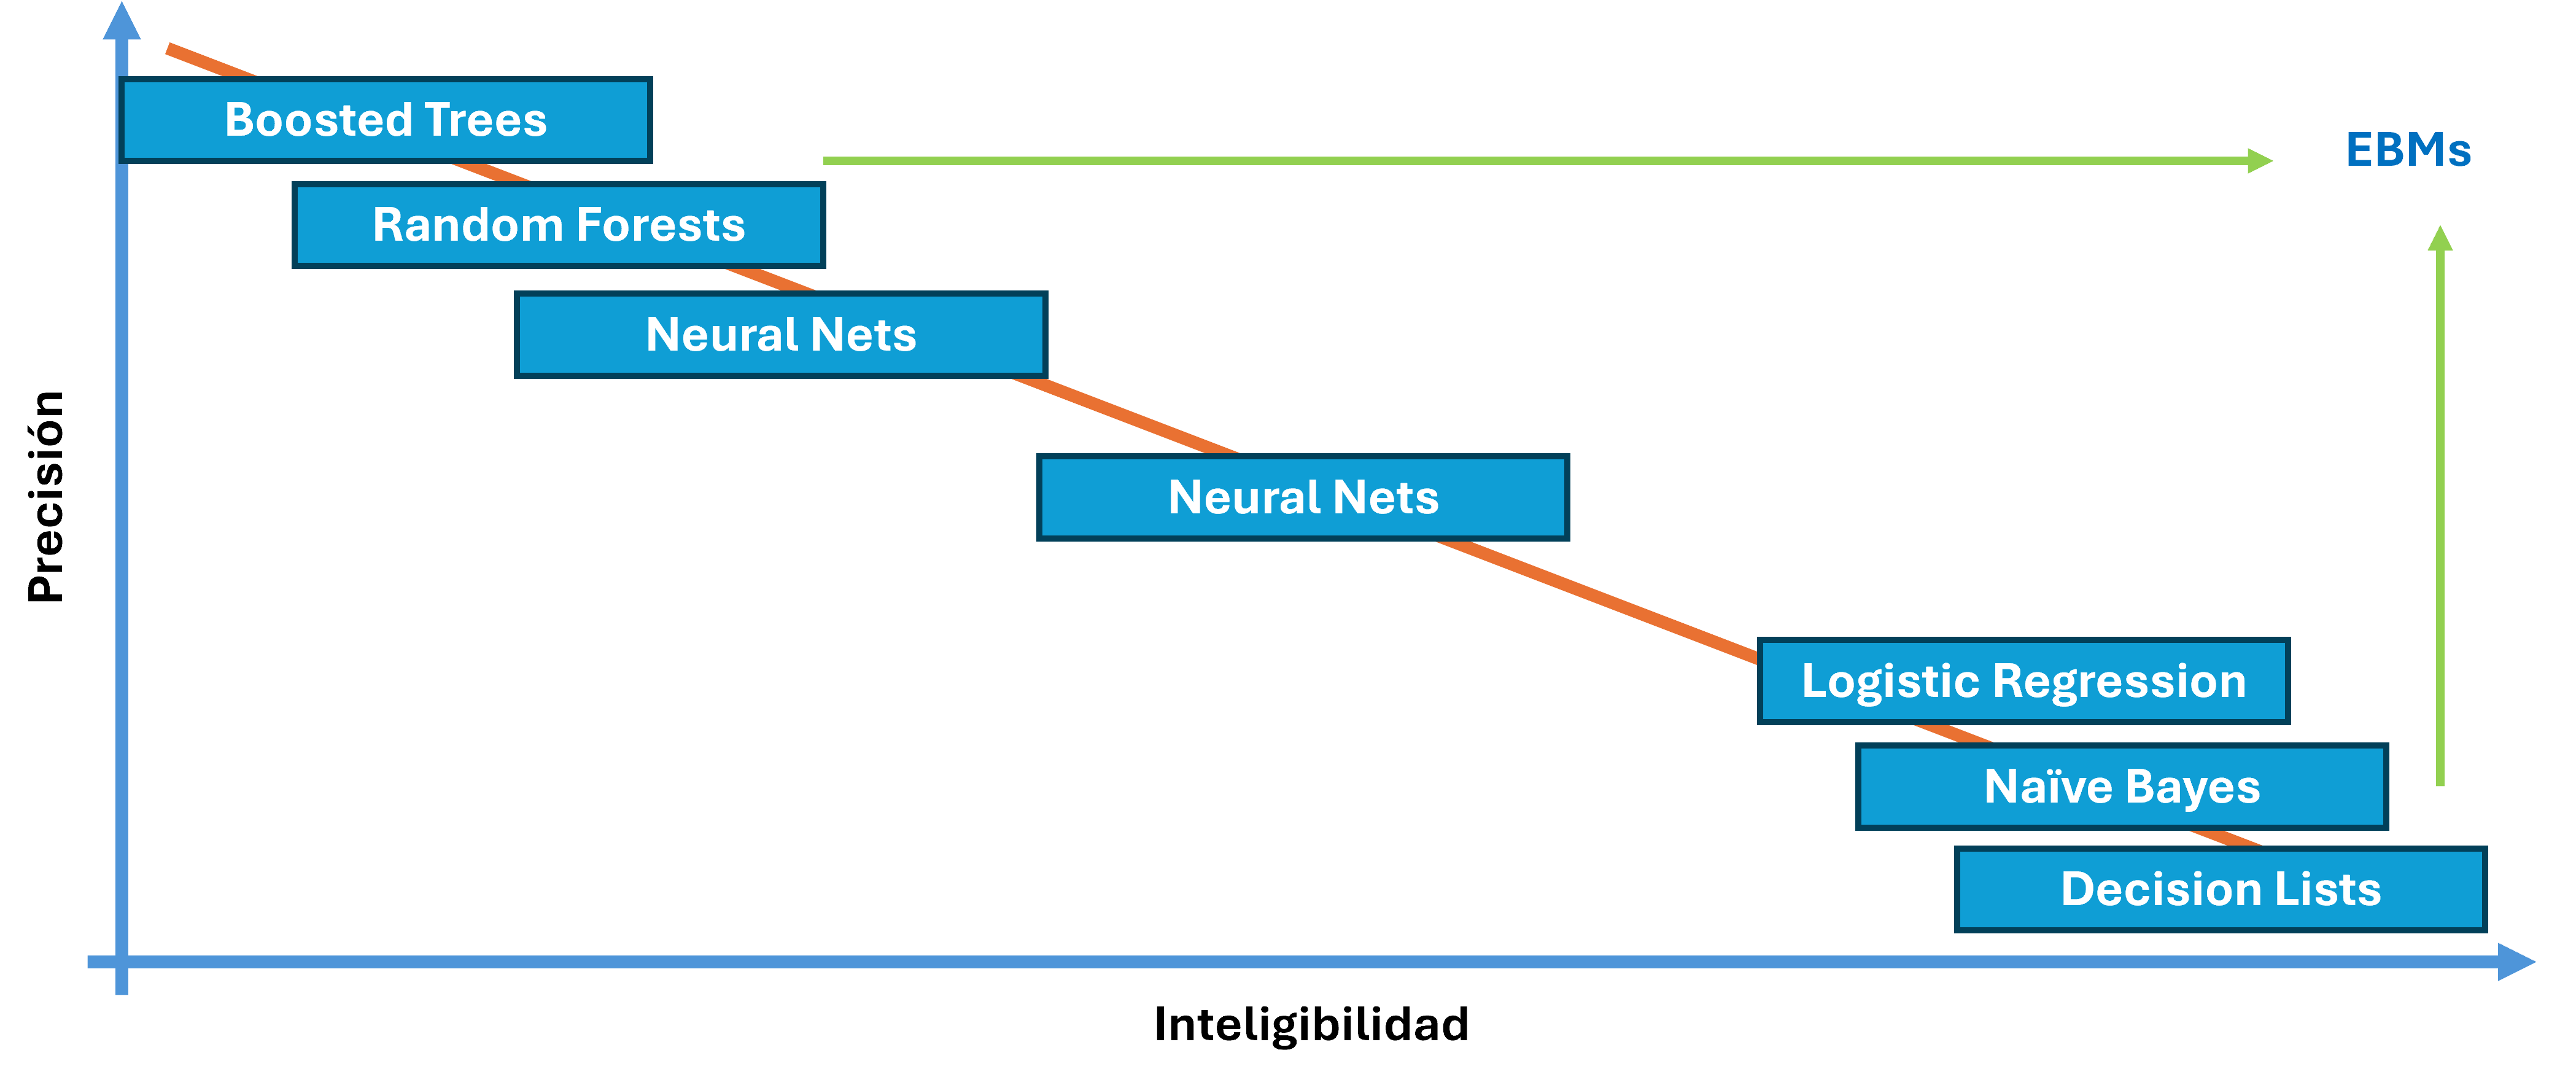
\includegraphics[width=0.9\textwidth]{include/EBMs.png}
    \caption{Gráfico comparativo de precisión e inteligibilidad de modelos de aprendizaje automático, inspirado en un gráfico presentado por \cite{microsoftEBMvideo}.}
    \label{fig:EBMs}
\end{figure}

El EBM es modular y permite visualizar cómo cada característica influye en las predicciones, facilitando la comprensión para los usuarios mediante gráficos claros, como los mostrados en la Figura \ref{fig:modularidad_ebm}, que ilustran la descomposición de una predicción individual y cómo cada característica contribuye de forma independiente.

InterpretML presenta varias ventajas:
\begin{itemize}
    \item Facilidad de comparación: La API unificada facilita la comparación de diferentes algoritmos de interpretabilidad, con integración sencilla a frameworks como scikit-learn.
    \item Interoperabilidad: Es compatible con herramientas como Jupyter Notebook y plotly, permitiendo una interacción intuitiva con los modelos y sus explicaciones.
    \item Visualización interactiva: InterpretML ofrece un panel de control interactivo que permite explorar visualmente las explicaciones generadas, ayudando a los usuarios a entender fácilmente las contribuciones de cada característica.
\end{itemize}

InterpretML ha demostrado ser útil en áreas como la salud, las finanzas y la justicia, donde la interpretabilidad es crítica. Su capacidad para combinar precisión y transparencia lo convierte en una herramienta esencial en sistemas de alta responsabilidad.

\subsection{Yellowbrick}

Yellowbrick es una biblioteca de visualización diseñada para facilitar la evaluación e interpretación de modelos de aprendizaje automático creados con scikit-learn. Esta herramienta ofrece una amplia gama de visualizaciones que permiten a los usuarios entender mejor el comportamiento de los modelos, ayudando en la toma de decisiones y mejorando la interpretabilidad de los mismos \cite{bengfort_yellowbrick_2018}.

\begin{figure}[H]
        \centering
        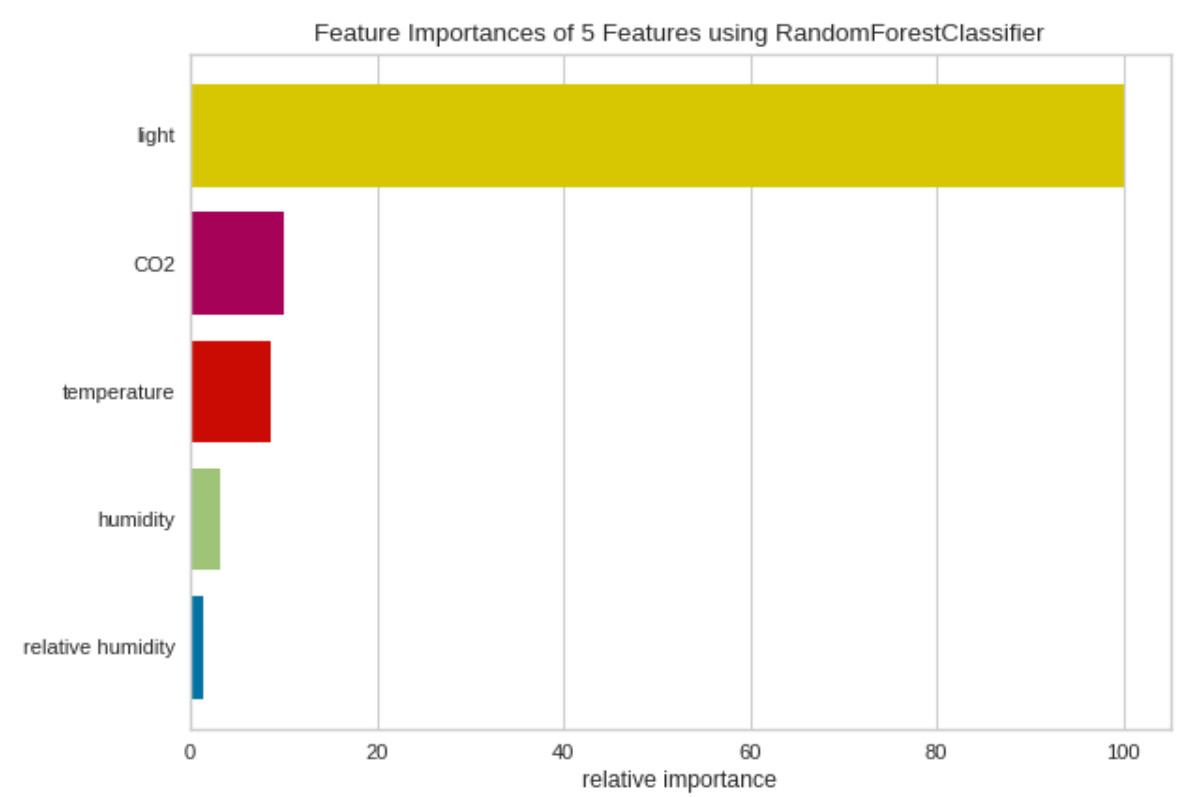
\includegraphics[width=0.8\textwidth]{include/yellowbrick.png}
        \caption{Visualización de la importancia de características generada por Yellowbrick utilizando un modelo \textit{RandomForestClassifier}. El gráfico muestra la influencia relativa de cinco características sobre las predicciones del modelo. La característica 'light' tiene la mayor importancia relativa, seguida de 'CO2' y 'temperature', lo que indica su fuerte contribución a las decisiones del modelo \cite{bengfort_yellowbrick_2018}.}
        \label{fig:yellowbrick_importance}
    \end{figure}

Yellowbrick se enfoca en generar gráficos que muestran cómo las características y el rendimiento de los modelos afectan los resultados, lo cual es esencial para los modelos transparentes como los Árboles de Decisión (DT) y los Conjuntos de Decisión Interpretables (IDS) utilizados en este trabajo. Entre sus funcionalidades más destacadas se incluyen:

\begin{itemize}
    \item \textit{Visualización de la importancia de características}: Yellowbrick permite representar gráficamente la importancia relativa de las características dentro de un modelo, como se muestra en la Figura \ref{fig:yellowbrick_importance}. En este TFM, esta herramienta es fundamental para comprender el impacto de las distintas características en las predicciones de los modelos de decisión. En particular, se ha empleado para identificar las características más influyentes dentro del dataset de matemáticas utilizado en este proyecto.
    
    \item \textit{Curvas de validación y curvas de aprendizaje}: Estas curvas permiten observar cómo el rendimiento del modelo varía según los valores de los hiperparámetros y cómo mejora a medida que recibe más datos de entrenamiento. Este tipo de visualización es útil para diagnosticar problemas de sobreajuste o subajuste, los cuales pueden afectar la interpretabilidad del modelo en este trabajo.

    \item \textit{Matrices de confusión y reportes de clasificación}: Facilitan la visualización de cómo el modelo clasifica correctamente e incorrectamente las instancias, lo que ayuda a comprender mejor el comportamiento del modelo en cada clase. Esta herramienta ha sido utilizada en este proyecto para analizar los resultados de los modelos DT y evaluar sus predicciones en relación con los datos de rendimiento académico en matemáticas.

    \item \textit{Curvas ROC y AUC}: Permiten evaluar el rendimiento de los modelos de clasificación, mostrando el compromiso entre la tasa de verdaderos positivos y la tasa de falsos positivos en diferentes umbrales de decisión. Estas curvas son especialmente útiles para evaluar la capacidad de los modelos para manejar errores de clasificación.
\end{itemize}

Yellowbrick ofrece ventajas significativas, entre las que destaca su integración perfecta con scikit-learn, lo que permite a los usuarios generar visualizaciones sin una configuración adicional compleja. Además, proporciona una interfaz fácil de usar que se adapta tanto a principiantes como a expertos, facilitando la evaluación visual de los modelos de manera clara y concisa.

\subsection{Anchors}

Anchors, propuestos por \textcite{ribeiro2018anchors}, son reglas locales que explican predicciones individuales de un modelo a través de condiciones suficientes. Estas reglas aseguran que si las condiciones de un \textit{anchor} se cumplen, la predicción del modelo será la misma con alta probabilidad. Los \textit{anchors} son especialmente útiles en modelos de caja negra o en tareas donde la interpretabilidad es fundamental. Aunque en este trabajo no implementamos \textit{Anchors}, su relevancia para el campo de la IA explicable es notable, ya que proporcionan explicaciones simples y de alta precisión que son fácilmente comprensibles por los usuarios.

En la siguiente tabla se muestra un ejemplo adaptado del artículo original, donde se utiliza \textit{Anchors} para etiquetar la parte del discurso de la palabra "play" en diferentes contextos.

\begin{table}[H]
    \centering
    \scriptsize % Reduce el tamaño de la fuente
    \renewcommand{\arraystretch}{1.5} % Ajusta el espaciado entre filas
    \begin{tabular}{p{4cm} p{5.5cm} p{3.2cm}}
        \toprule
        \textbf{Instancia} & \textbf{Condición} & \textbf{Predicción} \\
        \midrule
        I want to play(V) ball. & La palabra previa es \textbf{PARTICLE} & play es \textbf{VERBO}. \\ 
        I went to a play(N) yesterday. & La palabra previa es \textbf{DETERMINANTE} & play es \textbf{SUSTANTIVO}. \\ 
        I play(V) ball on Mondays. & La palabra previa es \textbf{PRONOMBRE} & play es \textbf{VERBO}. \\
        \bottomrule
    \end{tabular}
    \caption{Ejemplo de Anchors para la etiqueta de parte del discurso de la palabra "play" (adaptado de \textcite{ribeiro2018anchors}).}
    \label{tab:anchors-pos}
\end{table}


\noindent
En este ejemplo, el modelo predice si la palabra ``play'' es un verbo o un sustantivo dependiendo de la palabra que la precede, generando reglas locales que son fáciles de comprender y aplicar. Estos \textit{anchors} proporcionan una explicación clara sobre el comportamiento del modelo en casos específicos, lo que mejora la confianza y la interpretabilidad para los usuarios finales.



\subsection{DiCE: Explicaciones Contrafactuales Diversas}

DiCE (\textit{Diverse Counterfactual Explanations}) es un marco propuesto por \textcite{mothilal2020dice} para generar explicaciones contrafactuales que ayuden a los usuarios a comprender el comportamiento de modelos de aprendizaje automático. DiCE se centra en proporcionar múltiples explicaciones contrafactuales diversas, que exploran varias formas en las que se podría modificar una instancia para obtener una predicción diferente. Este enfoque permite a los usuarios entender qué cambios mínimos en los atributos de entrada podrían alterar la decisión del modelo, haciendo que este sea más interpretable.

Una \textit{explicación contrafactual} responde a la pregunta: “¿Qué habría que cambiar en esta instancia para obtener un resultado diferente?”. DiCE es capaz de generar varias explicaciones contrafactuales que muestran diferentes caminos posibles para lograr un cambio en la predicción. Esto es particularmente útil cuando hay varias combinaciones de características que pueden influir en el resultado, ya que proporciona al usuario un conjunto diverso de escenarios.

DiCE se basa en los siguientes principios:

\begin{itemize}
    \item \textit{Diversidad}: DiCE no genera una única explicación contrafactual, sino varias. Cada una ofrece una manera diferente de alterar la predicción de un modelo. Esta diversidad es útil para evitar que el usuario se enfoque solo en una explicación que podría no ser la mejor o más factible.
    \item \textit{Flexibilidad}: Los usuarios pueden especificar qué características se pueden cambiar y cuáles no. Esto es útil en casos donde ciertos atributos son fijos (por ejemplo, la edad de una persona) y no pueden ser modificados en las explicaciones contrafactuales.
    \item \textit{Compatibilidad con modelos de caja negra}: DiCE es un enfoque agnóstico al modelo, lo que significa que puede ser aplicado a una variedad de modelos, incluidos los modelos de caja negra.
    \item \textit{Optimización}: DiCE utiliza un algoritmo de optimización para generar explicaciones que minimizan el número de cambios necesarios en la instancia original. De esta forma, se realizan interpretaciones más realistas y fáciles de entender.
\end{itemize}

DiCE emplea un enfoque basado en la búsqueda de ejemplos contrafactuales cercanos que resulten en un cambio en la predicción del modelo. Dados los inputs de una instancia $x$ y una predicción del modelo $f(x)$, DiCE busca generar nuevos ejemplos $x'$ que pertenezcan a una clase diferente y que estén lo más cerca posible de la instancia original. Para lograr esto, DiCE resuelve el siguiente problema de optimización:

\[
\min_{x'} \, d(x, x') \quad \text{sujeto a} \quad f(x') \neq f(x)
\]

donde $d(x, x')$ es una métrica de distancia que asegura que los ejemplos contrafactuales sean similares a la instancia original. El objetivo es generar instancias contrafactuales $x'$ que difieran lo menos posible de $x$ y que den lugar a una predicción diferente por parte del modelo $f$.

Como ejemplo, consideremos un modelo de predicción de aprobación de préstamos. Si el modelo predice que un cliente no será aprobado para un préstamo, DiCE puede generar múltiples explicaciones contrafactuales mostrando qué atributos del cliente deben cambiarse para que la solicitud sea aprobada. Por ejemplo, una explicación podría sugerir que aumentando los ingresos anuales y reduciendo la deuda actual, el cliente podría obtener una aprobación. Otra explicación podría sugerir que reducir el número de créditos activos mejoraría las probabilidades de aprobación.

\begin{table}[H]
    \centering
    \scriptsize
    \renewcommand{\arraystretch}{1.5}
    \begin{tabular}{p{4cm} p{4cm} p{4cm}}
        \toprule
        \textbf{Atributo Original} & \textbf{Atributo Modificado (Contrafactual 1)} & \textbf{Atributo Modificado (Contrafactual 2)} \\
        \midrule
        Ingresos anuales: \$35,000 & Ingresos anuales: \$50,000 & Ingresos anuales: \$35,000 \\
        Deuda actual: \$10,000 & Deuda actual: \$5,000 & Deuda actual: \$10,000 \\
        Créditos activos: 3 & Créditos activos: 3 & Créditos activos: 1 \\
        \bottomrule
    \end{tabular}
    \caption{Ejemplo de explicaciones contrafactuales generadas por DiCE para un modelo de aprobación de préstamos. Se muestran múltiples combinaciones de atributos que podrían llevar a una predicción diferente.}
    \label{tab:dice-example}
\end{table}

Aunque DiCE es eficaz para generar explicaciones contrafactuales diversas, no garantiza que todas las explicaciones sean factibles o realistas en un contexto del mundo real. Por ejemplo, en el caso de la predicción de préstamos, aumentar los ingresos anuales puede no ser una opción viable a corto plazo para muchos individuos. Por lo tanto, es crucial que los usuarios de DiCE evalúen la plausibilidad de las explicaciones generadas.

DiCE es una herramienta poderosa para la IA explicable, permitiendo a los usuarios explorar cómo pequeños cambios en las entradas pueden alterar los resultados del modelo, y proporcionando una visión más completa del comportamiento del modelo a través de explicaciones diversas.



\section{Resumen}

En este estado del arte se han revisado las principales herramientas y enfoques de XAI, con especial énfasis en los modelos transparentes. También, se han explorado herramientas clave como InterpretML y Yellowbrick, que permiten visualizar y analizar la interpretabilidad de estos modelos, facilitando su comprensión por parte de los usuarios.

Asimismo, se han discutido métodos como Anchors, que proporciona reglas locales explicativas, y DiCE, que genera explicaciones contrafactuales diversas, destacando cómo estas técnicas ayudan a mejorar la transparencia y confianza en las predicciones de los modelos.

Esta revisión proporciona una base teórica sólida para el desarrollo del cuestionario de evaluación de interpretabilidad en este TFM, identificando los enfoques más relevantes para medir cómo los usuarios perciben la interpretabilidad de los modelos utilizados.

\chapter{Metodología}

En esta sección se describe la propuesta de este TFM, que consiste en el desarrollo de una herramienta de evaluación de la interpretabilidad basada en dos modelos: Árboles de Decisión (DT) y Conjuntos Interpretables de Decisión (IDS). La evaluación se realiza a través de un cuestionario implementado en una aplicación web diseñada para recolectar las respuestas de los usuarios y su percepción sobre la interpretabilidad de los modelos. Se explica el dataset utilizado para el entrenamiento de los modelos y generación de las preguntas del cuestionario. 

El código de implementación de los modelos, el preprocesamiento de datos y el análisis de interpretabilidad se encuentra en un notebook de Google Colab disponible en \cite{vargas2024interpretability}, donde se detallan todos los pasos involucrados en el proceso.


\section{Datos utilizados}

El conjunto de datos utilizado proviene del \textit{UCI Machine Learning Repository} es \cite{cortez2014student} y recoge información académica, social y demográfica de estudiantes de secundaria en dos escuelas portuguesas, centrado en las asignaturas de Matemáticas y Lengua Portuguesa. En este trabajo, solo se considera la asignatura de Matemáticas.

Este conjunto de datos es adecuado para evaluar la interpretabilidad de los modelos de clasificación debido a la variedad de características sociales, demográficas y académicas que pueden influir en el rendimiento académico. Además, la estructura del problema como una tarea de clasificación binaria permite una evaluación clara de los modelos propuestos en términos de su capacidad para predecir el éxito o fracaso de los estudiantes en la asignatura de Matemáticas.

Para la selección de las variables clave utilizadas en la construcción de los modelos, se realizó un análisis exploratorio tanto basado en la literatura \cite{cortez-2014} como en un análisis propio del dataset. El conjunto de datos original contiene un total de 33 características, que incluyen variables demográficas, sociales y académicas de los estudiantes. Inicialmente, se consideraron variables relacionadas con el desempeño académico, como \textit{G1}, \textit{G2} y \textit{G3}, que corresponden a las calificaciones parciales y final en la asignatura de Matemáticas. Sin embargo, se decidió excluirlas por las siguientes razones:

\begin{itemize}
    \item \textit{G3}: Esta variable representa la calificación final en Matemáticas y fue utilizada como la variable objetivo o dependiente en los modelos predictivos. Por lo tanto, no puede ser considerada como una variable predictora, ya que su valor es lo que se pretende predecir.
    
    \item \textit{G2 y G1}: Aunque estas variables corresponden a las calificaciones parciales en Matemáticas, se decidió excluirlas debido a su alta correlación con la variable \textit{G3}. Incluir estas variables podría sesgar el modelo hacia una predicción directa basada en estas notas, lo que no aporta valor en términos de interpretabilidad. Además, el objetivo de este trabajo es evaluar la interpretabilidad de los modelos basados en características externas, como las demográficas y sociales, y no únicamente en las calificaciones previas.
\end{itemize}

Para evaluar la importancia de las características seleccionadas, se utilizó un modelo de Árbol de Decisión (Decision Tree, DT), implementado mediante la librería \textit{Yellowbrick}, que proporciona gráficos de \textit{Feature Importance} para visualizar la contribución de cada característica al rendimiento del modelo. Esta herramienta facilitó la validación de la selección de variables basada en su relevancia predictiva. En la Figura \ref{fig:feature-importance} se muestra la importancia relativa de cada característica dentro del modelo DT.

\begin{figure}[H]
    \centering
    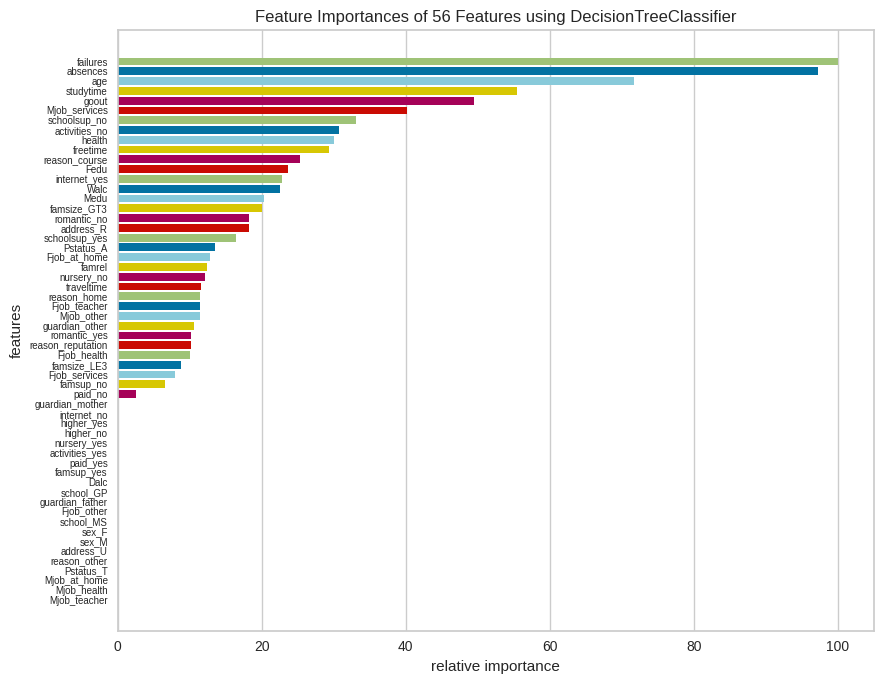
\includegraphics[width=0.95\textwidth]{include/importance_features.png}
    \caption{Importancia de las características calculada con \textit{Yellowbrick} para el modelo de clasificación utilizando Árboles de Decisión (DT). Las variables seleccionadas fueron validadas en base a su impacto en la predicción de la calificación final en matemáticas (\textit{G3}).}
    \label{fig:feature-importance}
\end{figure}

Para los modelos, se seleccionaron cuatro variables clave por su interpretabilidad y relevancia predictiva, basadas en el estudio de \cite{cortez-2014} y un análisis propio. Estas variables se detallan en el Cuadro \ref{tab:math-data-vars}.

\begin{table}[H]
    \centering
    \begin{tabular}{ll}
        \toprule
        \textbf{Característica} & \textbf{Descripción} \\
        \midrule
        \textit{absences} & Ausencias del estudiante en el año académico. \\
        \textit{failures} & Materias reprobadas en cursos previos. \\
        \textit{studytime} & Tiempo de estudio semanal: \\
            & 1: Menos de 2 horas \\
            & 2: 2 a 5 horas \\
            & 3: 5 a 10 horas \\
            & 4: Más de 10 horas \\
        \textit{age} & Edad del estudiante. \\
        \midrule
        \textit{G3} & Calificación final en Matemáticas. \\
        \bottomrule
    \end{tabular}
    \caption{Características seleccionadas para construir los modelos de predicción de rendimiento en Matemáticas, basadas en \cite{cortez-2014} y análisis propio. \textit{G3} es la variable dependiente.}
    \label{tab:math-data-vars}
\end{table}

El objetivo del modelo es predecir si un estudiante aprobará la asignatura de Matemáticas. Para esto, la variable \textit{G3} se convirtió en una variable categórica binaria, donde se considera \textit{Aprobado} cuando el estudiante obtiene una calificación final mayor o igual a 10 (en una escala de 0 a 20). La Tabla \ref{tab:math-data-clases} presenta la categorización de \textit{G3}.

\begin{table}[H]
    \centering
    \begin{tabular}{ll}
        \toprule
        \textbf{Clase} & \textbf{Definición} \\
        \midrule
        Aprobado & $G3 \geq 10$\\
        Reprobado & $G3 < 10$ \\
        \bottomrule
    \end{tabular}
    \caption{Clases creadas a partir de la calificación final (\textit{G3}) en Matemáticas, con un umbral de 10 puntos para definir Aprobado y Reprobado \cite{cortez2014student}.}
    \label{tab:math-data-clases}
\end{table}


\subsection{Implementación de los Modelos}
Para la evaluación de la interpretabilidad, se implementaron dos tipos de modelos:

\begin{itemize}
    \item \textit{Árboles de Decisión (DT):} Se utilizan por su facilidad de interpretación. Los Árboles de Decisión dividen el espacio de características mediante reglas simples, permitiendo a los usuarios visualizar cómo se toman las decisiones. Para su evaluación se emplean tanto métricas de precisión como análisis visual utilizando Yellowbrick.
    
    \item \textit{Conjuntos Interpretables de Decisión (IDS):} Los IDS se componen de reglas conjuntas que facilitan una explicación comprensible del modelo. En este trabajo, se evalúa su capacidad para generar decisiones claras y fáciles de entender para los usuarios.
\end{itemize}

















\subsection{Diseño del Cuestionario}
El cuestionario fue diseñado para recoger la percepción de los usuarios sobre la interpretabilidad de los modelos descritos anteriormente. Las preguntas fueron clasificadas en las siguientes categorías:

\begin{itemize}
    \item \textit{Preguntas de Precisión:} Los usuarios deben decidir si el modelo ha realizado una predicción correcta con base en las observaciones proporcionadas.
    \item \textit{Detección de Errores:} Los usuarios deben identificar si el modelo puede haber cometido un error en la predicción.
    \item \textit{Descripciones Generales:} Se pide a los usuarios que describan en sus propias palabras las reglas que los modelos han generado, permitiendo evaluar si el conjunto de reglas es comprensible.
\end{itemize}

\subsection{Desarrollo de la Aplicación Web}
La aplicación web fue desarrollada utilizando \textit{Flask}, un microframework de Python, y se aloja en la plataforma Railway. El flujo de trabajo de la aplicación es el siguiente:

\begin{enumerate}
    \item \textit{Carga de preguntas:} Las preguntas se almacenan en un archivo JSON, que es cargado y mostrado dinámicamente en la interfaz web.
    \item \textit{Recolecta de respuestas:} Cada respuesta del usuario se almacena en una base de datos MongoDB, junto con el tiempo que toma el usuario en responder cada pregunta.
    \item \textit{Procesamiento de resultados:} La aplicación genera un ID único para cada usuario y registra las respuestas para su posterior análisis.
\end{enumerate}

\subsection{Herramientas de Interpretabilidad}
Para facilitar el análisis de la interpretabilidad de los modelos, se emplearon dos herramientas principales:

\begin{itemize}
    \item \textit{InterpretML:} Se utilizó para generar explicaciones tanto locales como globales sobre las predicciones de los modelos implementados. El \textit{Explainable Boosting Machine (EBM)} también fue considerado para proporcionar un modelo más preciso y altamente interpretable.
    \item \textit{Yellowbrick:} Esta herramienta permitió visualizar la importancia de las características y generar gráficos como la curva ROC y la matriz de confusión, útiles para evaluar el rendimiento y la claridad de los modelos implementados.
\end{itemize}
